\section{Introduction}\label{introduction}

% Improving Locality of Unstructured Mesh Algorithms on GPUs

\noindent Unstructured mesh solvers, particularly applied to the solution of 
finite difference, finite volume or finite element algorithms, form the basis 
of numerical simulation applications in a vast area of important scientific 
domains, from modeling the flow of blood in the body, the flow past an aircraft, 
to ocean circulation and the simulation of Tsunamis. Significant computational 
resources are required for the execution of numerical algorithms on these highly 
detailed (usually three-dimensional) meshes. The solution involves repeatedly 
iterating over millions of elements (such as mesh edges, nodes, etc.) to reach 
the desired accuracy or resolution. The key distinguishing feature of these 
applications is that operations over mesh elements make use of explicit 
connectivity information between elements to access data defined on neighboring 
elements. This is in contrast to the use of stencils in structured-mesh 
applications where the regular geometry of the mesh implicitly provides the 
connectivity information. As such, iterations over unstructured-meshes lead to 
highly irregular patterns of data accesses over the mesh, characterized by 
indirect array accesses. For example, computations over the mesh involve 
iterating over elements of a set (e.g. faces), performing the same computations, 
on different data, accessing/modifying data on the set which they operate on 
(e.g. fluxes defined on the faces), or, using indirections accessing/modifying 
data defined on other sets (such as coordinate data on connected vertices). 
These indirect accesses are particularly difficult to parallelize when multiple 
threads may try to modify the same data, leading to data races. 

Previous work has utilized one of three approaches for handling data races 
during parallelization~\cite{LULESH:spec,miniaero}: (1) use coloring where the 
iteration set is ``colored'' such that no two iterations of the same color 
modify the same mesh element indirectly, followed by parallel execution of the 
iterations with the same color, (2) use large temporary datasets to stage 
increments without race conditions, and a separate step to gather the 
increments, or (3) use atomics to handle race conditions. However, the amount 
of parallelism, and especially the data locality available to be exploited with 
the above methods have become increasingly limited on modern and emerging 
massively parallel multi-core and many-core architectures. The performance gains 
have been limited particularly on many-core processors such as GPUs with 
thousands of low-power cores, but with modest memory-bandwidth. Thus, reducing 
data movement and exploiting memory locality during execution is vital on such 
devices. On GPUs, the first two techniques, coloring or using temporary 
datasets, end up with poor data locality as one cannot have good data reuse in 
both reading data as well as writing data without conflicts. The third method, 
atomics, are much more expensive operations than regular memory transactions and 
therefore usually lead to low throughput. 

In this paper we explore novel data-movement avoiding and locality exploiting 
algorithms for improving performance of unstructured-mesh applications on GPUs. 
Identifying that the throughput of memory transactions is the main bottleneck, 
we demonstrate how superior execution strategies can be obtained by utilizing 
a combination of techniques from (1) element reordering at thread-block level, 
(2) use of GPU shared memory as an explicitly managed cache and (3) use of 
partitioning algorithms for thread-block formation. We show how these allow us 
to maximize data re-use to the higher-bandwidth shared memory, and optimize 
access patterns to both shared and GPU global memory. More specifically, we make 
the following contributions:
\begin{enumerate}
\item We adopt a caching mechanism on the GPU that loads indirectly accessed 
elements into GPU shared memory. Then use a two-level ``hierarchical coloring'' 
approach to avoid data races, but improve locality over traditional global 
coloring. 

\item We design a reordering algorithm based on graph partitioning that 
increases data reuse within a thread block, also further increasing shared 
memory utilization. 

\item Finally, we apply the above techniques and optimizations to a number of 
representative unstructured-mesh applications to investigate performance on 
modern GPUs, contrasting performance improvements over the state-of-the-art. 
\end{enumerate}

\noindent We demonstrate how the above locality-exploiting algorithms provide 
performance improvements of up to 75\% compared to the state-of-the-art on the 
latest NVIDIA Pascal and Volta GPUs. The algorithms are implemented as an 
open-source software library~\cite{opt-library} and we illustrate 
its use for improving performance of existing or new unstructured-mesh 
applications.

The rest of the paper is organized as follows: the remainder of Section
\ref{introduction} introduces the basic concepts of unstructured meshes, 
numerical methods based on them and a discussion on related works, Section 
\ref{parallelisation-on-gpu} describes our optimized algorithms and the 
motivation leading to there design. Section \ref{performance} presents the 
performance analysis of the algorithms with experimental results. Finally, in 
Section \ref{conclusion}, we present conclusions from this research. 
\ref{library-implementation} contains a brief description of the structure of 
the open source library.


\subsection{Background}\label{sec:background}
\subsubsection{Unstructured meshes}\label{unstructured-meshes}

\noindent Unstructured meshes can be abstractly viewed as a collection of sets 
(e.g. nodes, edges, cells, etc.), data defined on these sets (e.g. fluxes, 
coordinates, velocities), and explicit connectivity information between 
sets. The connectivity information, declared as mapping tables are required for 
determining the neighbors of a set element. If we represent sets as consecutive 
indices from zero to the size of the set, then the mapping between two 
sets is represented as an array which stores the index of set elements in the 
second set of the mapping (referred to as the to-set) for every set element of 
the first set (known as the from-set). For the majority of such applications, the number of to-set elements connected to each from-set element is fixed (e.g. all edges have two vertices). For example consider the mesh illustrated 
in Figure~\ref{fig:unstructured}. Figure~\ref{fig:mapping} details how part of 
the mappings from edges to cells are defined for this mesh. Given such a 
mapping, we can access the index of those elements which are connected to the 
current element of the from-set from other sets (the to-sets of the mappings). 

The computations on the mesh are declared as a loop over the elements of a set, 
executing some block of computation on each set element (i.e. an elemental kernel), 
while accessing data directly on the iteration set or indirectly through a 
mapping.  If a loop over a set only write to data defined on that set during the 
elemental kernel, then each iteration of the loop could run in parallel. 
However, for kernels which indirectly increment data, there may be multiple 
from-set iterations that update the same to-set element. Such indirect-loops are 
common in finite volume and finite element applications over 
unstructured-meshes: e.g. when updating state variables in cells using fluxes 
across faces, or when doing matrix assembly. The parallelization of indirect 
loops are non-trivial as the exact elements leading to data races cannot be 
determined from compile time-information, given they are driven by the 
structure of the mesh in general and the mapping tables in particular, which are 
read in during run-time. 

% The sole focus of the research is this paper is this indirect-loop data access 
% pattern. 


\begin{figure}
\centering

\includegraphics[width=4cm]{fig/svg/unstructured.eps}
\caption{Unstructured mesh, the arrow represents the mapping tells $e_i$ is
  connected to $c_j$ and $c_k$.}
\label{fig:unstructured}
\end{figure}



\begin{figure}
\centering

\includegraphics[width=6cm]{fig/svg/mapping.eps}
\caption{A part of the mapping from edges to cells.}
\label{fig:mapping}
\end{figure}


Some restrictions that apply is also worth noting here. The first is the use of 
only a single level of mappings. This means that every piece of data that is 
accessed during an iteration over a set is either defined directly on that set, 
or is accessed through at most one level of indirection. However, this 
restriction does not exclude applications using nested indirections, since a 
mapping table can be created to contain the indexes that we access through 
multiple mappings. The second restriction is that the result of the operations 
on the sets are independent from the order of processing the elements of the 
sets (within machine precision). This restriction enables to exploit the 
maximum opportunities for parallelization given that the accuracy of the 
algorithms do not depend on the order of execution. Finally, only  mappings with 
a fixed number of connections (or arity) are considered; such as edges to 
vertices (where the degree is always 2), unlike for a vertices to vertices 
mapping, where this will vary. The natural formalization of most FEM and FV 
algorithm uses mappings with fixed number of connections.


\subsection{Related Work}\label{sec:related-works}
\noindent
Algorithms defined on unstructured meshes form an important 
class of applications at many organizations. It is one of the seven dwarfs -- 
common computation-communication patterns or motifs occurring in parallel 
numerical applications -- identified by Colella in 2004~\cite{Colella2004}. 
Discretizations such as finite volumes (FV) or finite elements (FE) often rely 
on these meshes to deliver high-quality results. Indeed there is a large number 
of papers detailing such algorithms, and a wide range of commercial, government, 
and academic research codes (e.g. OpenFOAM~\cite{OpenFoamUserGuide}, Rolls-Royce 
Hydra~\cite{moinier2002edge}, FUN3D~\cite{biedron2017fun3d}). All such 
applications use unstructured meshes in some shape or form, and are often used 
for large experiments, consisting of millions or even billions of mesh elements. 
These codes are generally critical to production and consume large portions of 
high-performance computing systems time. As such, the efficient execution of 
these applications on the parallel architectures of the day has been and 
continues to be crucial to the organizations and stake-holders that have 
invested in them for continued scientific delivery. Over the years, many works 
have discussed and presented techniques for efficient implementations, initially 
focusing on traditional CPU architectures~\cite{mavriplis2002parallel, 
jin1999openmp}, then many-core processors such as GPUs (as we discuss below), 
and even architectures such as FPGAs~\cite{nagy2014accelerating, 
akamine2012reconfigurable}. Many libraries have also been developed targeting 
unstructured-mesh solvers, from classical libraries~\cite{trilinos, PETSc} to 
domain specific languages~\cite{devito2011liszt, giles2012op2, pyfr2016}. 

The adoption of GPUs for these kind of computations has already led to 
considerable speedups over traditional CPU architectures due to the 
massive parallelism available on GPUs~\cite{Reguly2015, ELSEN200810148, 
cohen2009fast}. Other notable works have further looked at improving 
performance. Remacle et al. \cite{remacle2016gpu}, explores efficiently solving 
elliptic problems on unstructured hexahedral meshes on GPUs. They use shared 
memory for improving data locality, but advanced techniques, such as reordering 
and partitioning are not utilized. Work done by Castro et al. 
\cite{shallow_water} on implementing path-conservative Roe type high-order 
finite volume schemes to simulate shallow flows uses auxiliary accumulators to 
avoid data races while indirectly incrementing. Wu et al. 
\cite{wu2013complexity} introduce caching using the shared memory with 
partitioning (clustering), but do not use coloring. Instead they use a 
duplication method similar to that of LULESH and miniAero, as described below. 
Fu et al. \cite{fu2014architecting} also create contiguous patches (blocks) in 
the mesh to be loaded into shared memory, although they partition the nodes (the 
to-set) but not the elements (the from-set of the mapping). Furthermore, they do 
not load all data into shared memory, only what is inside the patch. Writing the 
result back to shared memory is done by a binary search for the column index and 
atomic adds, which leads to inefficiencies on the GPU. 

Parallel to the above work, the US Department of Energy labs have released a 
set of proxy applications that represent large internal production codes,
showing some of the computational and algorithmic challenges to be overcome on 
novel and emerging architectures Lulesh \cite{LULESH2:changes}, 
miniAero~\cite{miniaero}, BookLeaf~\cite{bookleaf}, MiniFE~\cite{minife}, 
PENNANT~\cite{pennant}. Out of this suite of codes there are three key 
approaches to handling data races: (1) allocate large temporary arrays where 
the intermediate results (i.e. the increments) are placed, avoiding any race 
conditions, followed by the use of a separate kernel to gather the results, 
(2) use atomics, (3) use coloring. These all lead to increased warp divergence 
and high data access latencies on GPUs; and the use of the temporary array also 
leads to more data allocations and movement, further constraining bandwidth. 

The research detailed in the present work is based on previous work 
in~\cite{op2}, where the OP2 library's GPU parallelization use shared memory on 
GPUs using CUDA for caching with a two level ``hierarchical'' coloring. However, 
we demonstrate superior execution strategies on GPUs with reordering of threads 
and data, to increase data reuse and maximize data locality. Instead of directly 
porting a specific application to use these techniques we present our methods 
as a classical library that can be used in general to accelerate unstructured 
mesh applications, and in particular the indirect increment algorithmic 
pattern, on GPUs. \textbf{[Is the utilization of this classical library 
presented in the paper given that we removed the appendix ? - Gihan]}

Most applications of interest for our work implements finite volume algorithms, 
and low order finite element algorithms, which has a lower computational 
intensity compared to the number of memory transactions. Thus our optimizations 
are targeted to avoid data movement, exploiting locality. In contrast high 
order finite element methods usually have significantly higher computational 
intensity, where there is a higher number of computations per data element 
accessed that can hide the cost of the memory access. While our techniques could 
potentially improve locality, memory bandwidth is less of a concern for such 
applications.


% In most finite volume algorithms, and low order finite element algorithms the 
% ratio of computations to number of bytes is relatively low - at least 
% compared to the ideal balance on modern GPUs. Therefore the proper usage of 
% the memory system for such simulations is crucial to get good performance. 
% High order finite elements usually have much higher computational 
% requirements, thus memory bandwidth is less of a concern. The throughput of 
% memory accesses is the main bottleneck for a large class of applications, thus 
% our goal is to lower the impact of the memory transactions. Since in most 
% applications of interest, there isn't enough computations to hide the cost of 
% memory movement, we can either increase the number of memory transactions in 
% flight (to more efficiently utilise bandwidth), or decrease the number of 
% memory transactions. To achieve the latter goal, a common technique is the use 
% of shared memory within CUDA thread blocks as an explicitly managed cache, 
% because it has much higher bandwidth and lower latency than global memory. The 
% challenge then is to maximise data re-use within shared memory, and optimise 
% access patterns to both shared and global memory.




\section{Parallelisation on GPUs}\label{parallelisation-on-gpu}

\noindent We begin by outlining the techniques used to effectively optimize 
unstructured mesh applications on GPUs -- some of which are well established 
and commonly used. We briefly show a na\"{i}ve solution, then continue 
with describing various improvements found in the literature, and then present 
our contributions.

\subsection{Traditional parallelization approaches}

\noindent On a GPU, groups of threads (warps) run at the same time, in 
lockstep. As such it is not efficient to execute computations of different 
length on different threads. Consequently, the usual practice is for each thread 
to take responsibility for the computation on one element of the set. This can 
be viewed as running one iteration per thread in the loop over a given set, also 
known as the iteration set or from-set. This allows the number of computations 
to be fixed, where the amount of data involved is fixed in the dimension of the 
mapping and the data arrays.

As mentioned before, care must be taken when writing parallel code to avoid 
data races when different threads modify the same data. There are three 
approaches discussed in the literature. The first is to color each thread 
according to the indirect data it writes, so that no two threads with the same 
color write the same data, and enforce ordering between colors using 
synchronization~\cite{Zegard2013}. On the GPU, one would do multiple kernel 
launches corresponding to the colors, so there is no concurrent writes between 
threads in the same kernel. We call this the \emph{global coloring} approach 
(Figure \ref{fig:unstructured_global}). The disadvantage here is that there is 
virtually no data reuse: when multiple elements write the same data, they are scheduled 
for execution in different launches. Since these operations also tend to read 
data through the same mappings, there is no data reuse in the reads either. 
Compounding the issue is low cache line utilization where elements of the same 
color are not neighbors in the mesh, and therefore unlikely to be stored in 
consecutive memory locations.

\begin{figure}[Htpb]
  \centering
  
\includegraphics{fig/svg/unstructured_global.eps}
  \caption{Schematic figure of the global colouring approach. In each kernel
  launch, the kernels work on edges of the same colour. The arrows
  represent the individual pieces of data loaded indirectly when executing the color red.}
  \label{fig:unstructured_global}
\end{figure}

The second approach is to serialize the indirect updates by means of locks or
atomic additions \cite{Kraus:2014:ACC:2691158.2691164}. This is considerably 
expensive on the GPU, since the whole warp has to wait at the synchronization 
step leading to warp divergence.

The third solution is the use of a large temporary array that stores the
results for each thread separately, avoiding race conditions by formulation 
\cite{LULESH:spec,miniaero}. However, after the computation finishes, a 
further kernel is required to gather the results corresponding to one data 
point. This suffers from the problem of not knowing how many values one thread 
has to gather, and as a result warps could diverge significantly, and 
memory access patterns are less than ideal. They can be good either for the 
write or the read, but not for both. Also, the size of the temporary array is the 
number of elements multiplied by the dimension of the mapping. As a result, it 
can be large, for example, in LULESH, it is \(8 \times 3 \times numElem \) 
in our measurements (where $numElem$ is the size of the from-set in LULESH), 
compared to the array defined on nodes where these values will ultimately end 
up, which is roughly the same as the number of elements themselves.

\subsubsection{Array-of-Structures (AoS) vs Structure-of-Arrays (SoA)} 
\label{aos-to-soa}

Due to the lockstep execution, consecutive threads in a warp read  memory at
the same time. Therefore, the layout of the data in the memory is an important
factor for performance. There are two commonly used
layouts~\cite{sharma2015data}: (1) Array-of-Structures (AoS) layout, where the
data associated with one element is in consecutive places in the array (and thus
in memory) and (2) Structure-of-Arrays (SoA) where the components of elements
are stored consecutively e.g. the first data component of the elements are in
the beginning of the array followed by the second, etc.

Although in most cases the SoA gives better performance on GPUs and better
vectorization on CPUs, the AoS layout is still commonly used on CPU
architectures with large caches. In the case of the AoS layout, consecutive
threads read data from strided addresses in memory and thus more cache lines 
are required to satisfy one transaction. This would be compensated by 
subsequently reading the other components, but may have a negative effect on 
 GPUs due to their small caches. Conversely, with the SoA layout, the 
threads read data next to each other, which means that the data needed by 
consecutive threads are most probably in the same cache line resulting in 
coalesced memory transactions. However, when indirections are involved, these
access patterns become more complicated --- even with the SoA pattern,
consecutive threads may not be reading consecutive values in memory, and
therefore cache line utilization degrades. The choice of data layout in
unstructured mesh computations is therefore highly non-trivial, as we show
later.

\subsection{Shared memory approach}\label{shared-memory-approach}

Considering the three data race avoiding approaches, we see that they all only 
make use of the GPU global memory. As such one technique to further improve 
performance is by reducing memory accesses to the GPU global memory. To this 
end, the OP2 library~\cite{op2} targets the use of the shared memory on the 
GPUs. Shared memory, is only shared within thread blocks, but has much lower 
access latency and higher bandwidth than the global memory. The idea is to 
collect the data required to perform the computations and load it into shared 
memory. Then, during computation, the indirect accesses are to the shared
memory, and the result can also be stored there. After computations by all 
threads in the block have completed, the contents of the shared memory can be 
written back to global memory. One immediate advantage of this approach is that 
the fetching and writing back of data from/to the global memory can be done by 
the threads independently of the actual threads that will be carrying out the 
computations on them. Particularly, reading/writing can be done in the order 
in which the data is laid out in memory, ensuring maximum utilization of 
cache lines. With the AoS layout, data can be read in contiguous chunks as 
large as the number of components in the structure.

The use of shared memory of course leads to one additional complication. 
Writing back the updated patches of shared-memory to GPU global memory may lead 
to data races. This leads to the use of a \emph{two-layered coloring} or 
\emph{hierarchical coloring}~\cite{op2} scheme. The blocks as well as the 
threads within a block is colored (Figure \ref{fig:unstructured_hier}). The 
former is to avoid data races when thread blocks write the result back to 
global memory and the latter is to avoid threads writing their results into 
shared memory at the same time. 

\begin{figure}[Htpb]
  \centering
  
\includegraphics{fig/svg/unstructured_hier.eps}
  \caption{Schematic figure of the hierarchical coloring approach. The thread
  blocks are circled with dashed lines. The arrows represent the individual 
  pieces of data loaded.}
  \label{fig:unstructured_hier}
\end{figure}

Algorithm~\ref{code:shared} details the steps carried out by a CUDA kernel for 
executing within this two-level coloring scheme. All indirect data accessed 
by the block (which is identified during a preprocessing phase) is fetched from 
global to shared memory to shared memory. Here, the operation consists of two 
nested loops: (1) an iteration over the data points, and within that, (2) an 
iteration over the data corresponding to the data point. For the SoA layout, 
only the outer loop needs to be parallelized, as this will cause parallel 
read operations to access memory addresses next to each other. For the same 
reason, if the AoS layout is used, both parallel loops need to be parallelized
(i.e. collapsed into one). The data layout in shared memory is best be set to SoA: 
our measurements showed a consistent degradation in performance when switching 
to AoS layout, due to the spatial locality described in Section 
\ref{aos-to-soa}: it leads to fewer bank conflicts.

After the data is loaded into shared memory, each thread executes the main body 
of the kernel, and outputs are placed into registers.  Next, the threads update 
the result in shared memory with their increments. Finally the updated data is 
written back to global memory.

\begin{algorithm}
  \begin{algorithmic}
    \State tid = blockIdx.x * blockDim.x + threadIdx.x
    \State bid = blockIdx.x
    \ForAll {d $\in$ indirect\_data}
      \State shared[shared\_ind(d)] = global\_indirect[d]
    \EndFor
    \State \_\_syncthreads()
    \State result = computation(shared[mapping[tid]], global\_direct[tid])
    \State \_\_syncthreads()
    \State fill shared with zeros
    \State \_\_syncthreads()
    \For {c = 1 $\ldots$ num\_thread\_colours}
      \If{c == thread\_colours[tid]}
        \State increment shared with result
      \EndIf
      \State \_\_syncthreads()
    \EndFor
    \ForAll{d $\in$ indirect\_data}
      \State increment global\_indirect\_out with shared
    \EndFor
  \end{algorithmic}
  \caption{Algorithm to use the shared memory to preload indirect data accessed
  within a thread block. \lstinline!global_indirect! holds the data indirectly
  read, \lstinline!global_indirect_out! holds the result of the iteration.}
  \label{code:shared}
\end{algorithm}

One other benefit from using shared memory with hierarchical coloring is the 
improved data reuse within the block. Each piece of data has to be loaded 
from global memory only once, but can be used by multiple threads (e.g. data on 
a shared edge between two triangles). However, the greater the reuse, the more 
thread colors we have: the number of colors is no less than the number of 
threads writing the same data. Since the number of synchronizations also grows 
with the number of thread colors (more precisely, it is the number of colors 
plus two, one before and one after the computation if the input and the 
increment are stored separately in shared memory), there is a trade-off between 
the number of synchronizations and data reuse. Our measurements showed that if 
the kernel is memory-bound, the greater data reuse leads to increased 
performance, but the trade-off is non-trivial, as we will demonstrate in 
Section~\ref{performance}.

\subsection{Increasing data reuse}\label{increasing-data-reuse}
\noindent Building on the shared-memory with hierarchical coloring, the first 
contribution of our work attempts to further increase data reuse through 
reordering of elements. Specifically, reordering of the elements in the
from-set (which map directly to the threads), allows us to control 
how CUDA thread blocks are formed and how much data reuse can be achieved. 
With the shared-memory approach, the benefit of data reuse is twofold: it 
decreases the number of global memory transactions and decreases the size of 
shared memory needed, which leads to greater occupancy. Two different 
approaches to re-ordering is explored (1) the sparse matrix bandwidth reducing 
Gibbs-Poole-Stockmeyer algorithm~\cite{gps} and (2) graph partitioning.

% In our measurements, we only consider one kernel and reorder accordingly. This
% does not affect the performance of direct kernels (kernels in which there is no
% indirect access), and---since data locality loosely corresponds to locality in
% the world of the physical computation being calculated---also helps other
% indirect kernels.

\subsubsection{Gibbs-Poole-Stockmeyer-based reordering}

\noindent For serial implementations of computations on graphs (typically on 
CPUs), the Gibbs-Poole-Stockmeyer algorithm (GPS,~\cite{gps}) is a heuristic 
algorithm that increases spatial and temporal locality when traversing the 
nodes. For example, considering a mesh with edges and nodes, where the edges are 
the elements of the from-set of the mapping, and the nodes form the to-set, GPS 
would renumber the nodes and change the order of traversal. The renumbering is 
done by going through the nodes in a breadth-first manner from two distant 
starting points, and then renumbers the nodes so that the levels of the 
resulting spanning trees will constitute contiguous blocks in the new 
permutation. After renumbering its points, which by design improves spatial 
locality, we order the edges of the graph lexicographically, so that consecutive 
threads (or spatial iterations in serial implementations) have a higher chance 
of accessing the same points, which improves temporal locality (data reuse). 
The algorithm can be generalized to meshes by transforming each element into a
fully connected graph of its points and then taking the union of these. An
example of this is shown on Figure \ref{fig:mesh2graph}.

\begin{figure}%
  \centering%
  \subfloat[][]{%
    \centering%
    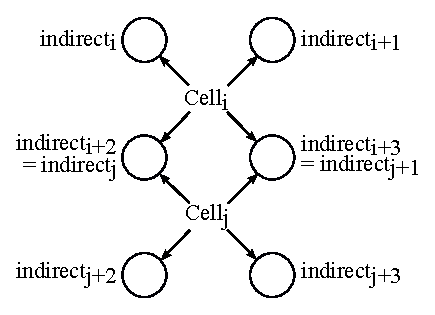
\includegraphics[width=5cm]{fig/svg/mesh2graph.eps}%
    \label{fig:mesh2grapha}%
    }%
  \qquad
  \subfloat[][]{%
    \centering%
    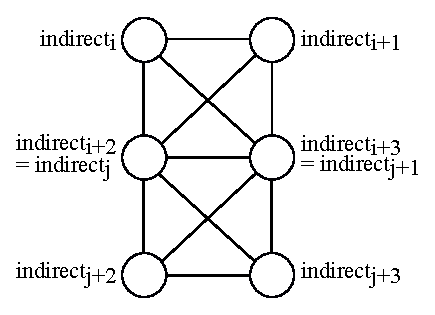
\includegraphics[width=5cm]{fig/svg/mesh2graph_graph.eps}%
    \label{fig:mesh2graphb}%
    }%
  \caption[]{An example of converting a mesh (shown in \subref{fig:mesh2grapha},
  with mapping dimension 4) to a graph (on Figure \subref{fig:mesh2graphb}) for
  the GPS algorithm.}%
  \label{fig:mesh2graph}
\end{figure}

There are several straightforward generalizations to handle multiple sets and
mappings (e.g. vertices, edges, cells and their connections).  The first is to
assume that all the mappings describe a similar topology, so the elements can be
reordered based on only one of the mappings (as described above), then reorder 
the points accessed through the other mappings by, for example, a greedy method.
Another approach could be to reorder every data set separately, and then reorder
the elements based on the new order of the accessed points, combining the
separate data sets (and corresponding mappings) in some way. Since the mappings
in the applications we measured are very similar topologically (in fact, except
for one of the applications we tested, Airfoil, there is only one mapping in 
each application), we used the first method. However, the algorithm fails to 
take into account that on the GPU the threads are grouped into blocks, and data 
reuse can only realistically be exploited within blocks. The next algorithm 
addresses this limitation.

\subsubsection{Partitioning based reordering}

\noindent To increase data reuse within a block is equivalent to decreasing 
data shared \emph{between} the blocks, more specifically, to decrease the 
number of times the same data is loaded in different blocks (see 
Figure~\ref{fig:unstructured_part}). With the shared memory approach, data needs 
to be loaded only once per block. So the task is to partition the elements into 
blocks of approximately the same size in such a way that when these blocks are 
assigned to CUDA thread blocks, the common data used (loaded into shared 
memory) by different blocks is minimized.

\begin{figure}[Htpb]
  \centering
  
\includegraphics{fig/svg/unstructured_part.eps}
  \caption{Schematic figure of the hierarchical colouring approach with
  partitioning. The thread blocks are circled with dashed lines. The arrows
  represent the individual pieces of data loaded; note that this is less than
  in Figure \ref{fig:unstructured_hier}.}
  \label{fig:unstructured_part}
\end{figure}

Let $G_M$ be a graph constructed from the original mapping, where the points are
the threads, and there is an edge between them if and only if they access the
same data, and let $P_{G_M} = \{B_1, \ldots, B_n\}$ be a partition of this graph
with $n$ blocks. This works even with multiple mappings. If there is a set of 
blocks $B_{d_1}, \ldots, B_{d_k}$ that access the same piece of data, then they 
form a clique in $G_M$ in the sense that between any pair of blocks $B_{d_i}$ 
and $B_{d_j}$ (where $1 \le i,j \le k$), there is an edge of $G_M$ between $u$ 
and $v$ such that $u \in B_{d_i} \wedge v \in B_{d_j}$. Note that the cliques 
have $0.5 \cdot (k^2 - k)$ edges, which is a monotone increasing function in 
$k$, since $k \ge 1$ (there is at least one block writing each data point, 
otherwise it is of no relevance). That means that partitioning using the usual 
objective of minimizing the number of edges between blocks is a good heuristic 
for maximizing data reuse within the blocks.

We chose the k-way recursive partitioning algorithm used by the 
METIS~\cite{metis} library to partition the graph $G_M$. It is a hierarchical
partitioning algorithm, where it first coarsens the graph by collapsing nodes, 
then partitions using the recursive bisection algorithm, and then finally while 
progressively un-coarsening the graph, locally optimizes the cuts. The algorithm 
attempts to maintain equal block sizes in the resulting partition, however, it 
is not always possible because of the underlying algorithm. Since CUDA launches 
thread blocks with equal size, this must be the maximum of the block sizes in 
the created partition. Consequently some threads do not do any work, 
lowering occupancy. One of the tuning parameters for the algorithm is the the 
load imbalance factor, which can be used to specify the tolerance for this 
difference. It is called load imbalance because METIS was originally used 
for distributing computation, ie. load, in a distributed memory system. The 
Load imbalance factor is defined as $l = n\max_j \left\{\mathrm{size}(B_j) 
\right\}$, where $n$ is the number of blocks and $\mathrm{size}(B_j)$ is the 
size of the $j$th block. Due to the local optimization in the un-coarsening 
phase, it is impractical to set this parameter to $1$ (meaning the block sizes 
must be exactly the same). We found that a tolerance of $1.001$ works well in 
practice for our needs.

We design the block size to be a tuning parameter, which specifies the actual
block size of the launched GPU kernels. The number of working threads
cannot exceed the block size. To account for this in partitioning, we calculate 
a new block size ($S'$) and tolerance ($l'$) with margins for the imbalance:
\begin{align}
  S' &= \left\lfloor \frac{S}{l} \right\rfloor \\
  l' &= \frac{S + \epsilon}{S'},
\end{align}
where $S$ is the original block size, $l$ is the original load imbalance
parameter and $\epsilon$ is an empirical tuning parameter to create as large
blocks (within the limit) as possible. This support for a variable number of 
working threads (ie. to determine if the current thread should do any actual 
computation) also incurs a slight overhead of having to load the start and end 
index for each block. We found this overhead to be minimal in practice.

Due to the way loads and stores work on the GPU, what actually affects
performance is not the number of data points accessed, but rather the number of
cache lines (of size 32 bytes on the hardware used) that are accessed. A simple 
heuristic reordering of data points is used to account for this. 

The idea is to group data points together (in a contiguous chunk of memory) that
are read/written by the same set of blocks: this makes them more likely to be
loaded in the same cache line. This is even more important when more blocks
access the same group of data points, since then inefficiencise will worsen
performance for each of these blocks. As a simple heuristic, we group data
points with the same number of blocks that access them together (by sorting),
and within these groups, we sort by the indices of the accessing blocks
lexicographically.

\subsection{Further optimizations}\label{optimisations}

\noindent There are a number of further optimizations we introduced to improve
performance. We can increase the number of loads or stores in flight 
to/from global memory by using CUDA's built-in vector types 
(\lstinline!float2!, \lstinline!float4! and \lstinline!double2!). This way, 
each thread will load multiple consecutive values from memory during a single 
transaction. This is useful to increase the efficiently of loads that are 
already coalesced.

When updating the shared memory with increments, the threads within a block can 
be sorted by their color. Then threads with the same color will be next to each 
other, so warps will have fewer threads of different colors. This results in 
reduced warp divergence on average.

Marking pointers to data on the GPU with \lstinline!__restrict__! and 
\lstinline!const! where applicable enables the compiler to apply further 
reordering optimizations, which it would not have deemed safe to do otherwise. 
\lstinline!__restrict__! instructs the compiler that the pointers do not 
\emph{alias} one another, ie. do not point to the same memory space. The 
\lstinline!const! enables the compiler to place the data in texture cache that 
has lower latency than the global memory.


\section{Library implementation}\label{library-implementation}

Deploying the locality exploiting algorithms developed in this research to 
existing and new unstructured-mesh applications is the subject of this appendix. 
The algorithms have been implemented as an open source library 
at~\cite{opt-library}. We first provide an overview of the re-engineering /
development process required to utilize the library followed by a step-by-step 
guide to the workflow involved. 

There are two primary concerns for deployment. First, given an existing 
application, its current data layout may need to change to accommodate AoS, SoA 
or reordering of mesh elements. Data layout reorganization has a one-off cost, and needs to be 
performed during initialization. Changing data-layouts between different 
computational kernels is usually prohibitively expensive and therefore avoided. 
Reordering will not affect direct kernels, but it will affect indirect kernels. 
AoS/SoA transformations affect all kernels. The impact of these transformations 
need to be considered as a whole on the applications. 

Secondly, the CUDA kernels that perform the computations need to be changed to 
load, process and store data as was described in 
Section~\ref{shared-memory-approach}. This will essentially involve directly 
modifying the computational kernels of the unstructured-mesh application we are 
deploying the optimizations to. The goal therefore is to minimize the amount 
of changes required to be done on the original code.

\textbf{Done up to here - Gihan}

% involve surrounding the computational kernel with code provided by our library. 

% \subsection{Integration into codes}

% There are two key components to deploying these transformations and 
% optimizations. First, the existing data layouts may need to be changed to
% accommodate AoS, SoA or reordering optimizations, and any auxiliary datasets
% need to be computed (e.g. exact block sizes when using partitioning-based
% reordering). Second, the CUDA kernels that perform the computations need to be
% changed to load, process and store data. The latter was described in Section
% \ref{shared-memory-approach} -- the computational kernel needs to be 
% surrounded by code provided by our library. Data reorganization and execution 
% planning has a one-off cost, and needs to be performed during 
% initialization---our library
% also provides these as functions. It can of course affect other parts of the
% code as well---as discussed above, reordering will not affect direct kernels,
% but it will affect indirect kernels, and AoS/SoA transformations affect all
% kernels. The impact of these transformations need to be considered as a whole 
% on the applications, considering re-organization between different 
% computational kernels is usually prohibitively expensive.


% In our library, the AoS--SoA transformation is governed by a tunable
% hyperparameter on a dataset-by-dataset basis. A hybrid SoA-AoS layout was not 
% considered, due to the fact that the library is designed to be integrated 
% into existing applicaitons, and the complexity


\subsection{User kernels}




The concept of a computation is in the form of a loop (or kernel) body. The loop
body is written by the user from a skeleton code, the library only calls it. The
same code can be used as in the serial algorithm, with the restrictions
described in Section \ref{unstructured-meshes} and with the modification that,
since the data layout is not necessarily the usual AoS, the accesses need to use
the stride parameters (supplied to the kernel by the library) that are defined
to be the distance between two consecutive data component (e.g. this will be $1$
in the case of AoS).

Four types of loops are supported: one serial and three parallel. The
parallelisations are done by (1) OpenMP on the CPU, (2) CUDA with global
colouring and (3) CUDA using the shared memory approach with hierarchical
colouring on the GPU. The CPU versions are not optimized and are only there for
testing and verification purposes. The user of the library can choose which of
these to apply.

The user kernel consists of two main levels. In the first, the pointers to the
data arrays are acquired, typecast and the result is written back into global
(GPU or CPU) memory. This is similar in the differently parallelised loops (e.g.
there is usually no difference between the serial and the OpenMP versions), but
there are small variations in the use of GPU shared memory, the synchronization
steps and the calculation of the loop variable. (By loop variable, we mean the
index from the from-set.) In our current implementation, the user creates this
level from provided templates, but this can be easily automated by means of a
source-to-source translator tool. The second level is the calculation itself
that should be the same for all loop forms.

The data will be automatically copied to the device before the beginning of the
loop when the program is running on the GPU, and the result will be copied back
to the host after. The pointers supplied to the user kernel also point to the
location in the appropriate address space.

Data accessed only directly is always in SoA form, while the layout of the
data indirectly accessed is a user supplied compile time parameter. The layout
of the shared memory is determined by the user; it is SoA in the kernels in our
measurements. The layout of the mappings is AoS for all the parallelisation
methods except hierarchical colouring.

In the case of OpenMP and global colouring, the parallel execution is
synchronized by the library using multiple kernel launches. The hierarchical
colouring has some additional synchronization steps, as described by Algorithm
\ref{code:shared} in Section \ref{shared-memory-approach}.

\subsection{Execution planning}

We use colouring to avoid data races. Two kinds of colouring algorithms are
used: global colouring is used for the OpenMP and the first CUDA
parallelisation, while hierarchical or two-layer colouring is used for the
shared memory approach.

The global colouring is a direct generalization of the greedy graph colouring
algorithm: for all elements of the from-set, its colour will be one of those
that are used but none of its corresponding indirect points have.

The threads with different colours are started in different kernel launches. The
mappings and the direct accessed data arrays are reordered according to their
colour, so there is no need for another indirection.

If partitioning is used in the preprocessing step, the hierarchical colouring
reorders the threads according to that and maps the threads to blocks. The block
sizes are limited by a parameter (given by the user), and if the partitioning
algorithm produced a block that is larger, it is divided into two CUDA blocks.

The same greedy colouring algorithm described above is then used to colour the
thread blocks. Within the blocks we use the heuristics of ordering the threads
by removing the one with the minimum degree, placing it last in the ordering,
then recursively ordering the other threads.

After colouring the threads are sorted according to their colour to reduce warp
divergence, as described in Section \ref{optimisations}.

The mappings and the direct accessed data are transformed into SoA layout to
increase spatial locality. Similarly to the global colouring, these are then
reordered so they can be directly indexed by the loop variable.

\subsubsection{Reordering}

Before the execution of the loop an optional preprocessing step is to either
reorder the from- or to-set elements using the GPS algorithm, or map the threads
to blocks by a partitioning algorithm described in Section
\ref{increasing-data-reuse}.

We use the Scotch library\cite{scotch} for the GPS algorithm, and the
METIS\cite{metis} library for the multilevel k-way partitioning algorithm (using
64 bit integers for indices). We also tried the recursive bisection algorithm in
the METIS library, but the result was significantly worse, as well as the
partitioning algorithm in the Scotch library, but that failed to stay within
tolerance (and half of the blocks in the partition were empty, others were
larger then requested).

% vim:set et sts=2 sw=2 ts=2 tw=80:


\section{Measurements}\label{measurements}

\subsection{Used applications}\label{used-applications}
\subsubsection{Airfoil}
Airfoil is a benchmark application, representative of
large industrial Finite Volume CFD applications. It is a non-linear 2D inviscid
airfoil code that uses an unstructured grid and a finite-volume discretisation
to solve the 2D Euler equations using a scalar numerical dissipation. The
algorithm iterates towards the steady state solution, in each iteration using a
control volume approach, meaning the change in the mass of a cell is equal to
the net flux along the four edges of the cell, which requires indirect
connections between cells and edges. Airfoil is implemented using the OP2 domain
specific language \cite{op2}, where two versions exist, one implemented with
OP2's C/C++ API and the other using OP2's Fortran API
\cite{giles2012op2,op2-repo}.

The application consists of five parallel loops: \textbf{save\_soln},
\textbf{adt\_calc}, \textbf{res\_calc}, \textbf{bres\_calc} and \textbf{update}.
In our work we focus on \textbf{res\_calc} since it has indirect increments and
about the 70\% of the time is spent in this kernel on GPUs with global
colouring.  This is the most complex loop with both indirect reads and writes; it
iterates through edges, and computes the flux through them. It is called 2000
times during the total execution of the application and performs about 100
floating-point operations per mesh edge. In each iteration, it reads 5 and
increments 4 double values from each of the 2 indirectly accessed cells, and
reads 2 double values from each of the 2 indirectly accessed nodes.
\\
 The tests are executed on a mesh containing 2.8 million cells.

\subsubsection{Volna}
Volna is a shallow water simulation capable of handling the complete life-cycle
of a tsunami (generation, propagation and run-up along the coast)
\cite{dutykh2011volna}. The simulation algorithm works on unstructured
triangular meshes and uses the finite volume method. Volna is written in C/C++
and converted to use the OP2 library\cite{op2}. For Volna top three kernels
where most time is spent: \textbf{computeFluxes}, \textbf{SpaceDiscretization}
and \textbf{NumericalFluxes}. We focus on the \textbf{SpaceDiscretization}
kernel since it has indirect increments and the 60\% of the time spent inside
this step on GPU with global colouring. In each iteration,
\textbf{SpaceDiscretization} reads 1 and increments 4 float values from each of
the 2 indirectly accessed cells, and reads 7 float and 1 integer values directly.

Tests are executed in single precision, on a mesh containing 2.4 million
triangular cells, simulating a tsunami run-up to the US pacific coast. The
kernel itself iterates over the edges and increments the cells.

\subsubsection{BookLeaf}
BookLeaf is a 2D unstructured mesh Lagrangian hydrodynamics application from the
UK Mini-App Consortium \cite{uk-mac}. It uses a low order finite element method
with an arbitrary Lagrangian-Eulerian method.  Bookleaf is written entirely in
Fortran 90 and has been ported to use the OP2 API and library. Bookleaf has a
large number of kernels with different access patterns such as indirect
increments similar to increments inside \textbf{res\_calc} in Airfoil. For
testing we used the SOD testcase with a 4 million element mesh. The top three
kernels with the highest runtimes are \textbf{getq\_christiensen1},
\textbf{getacc\_scatter}, \textbf{gather}. Among these there is only
one kernel (\textbf{getacc\_scatter}) with indirect increments so we tested our
optimisations on this kernel. This kernel reads 17 double values directly, and
increments 4 double values on each of the 4 indirectly accessed nodes in each
iteration.

\subsubsection{miniAero}\label{sec:mini-aero-summary}

miniAero \cite{miniaero} is a mini-application for the evaulation of programming
models and hardware for next generation platforms from the Mantevo suite
\cite{heroux2009improving}. MiniAero is an explicit (using 4th order
Runge-Kutta) unstructured finite volume code that solves the compressible
Navier-Stokes equations. Both inviscid and viscous terms are included. The
viscous terms can be optionally included or excluded. For miniAero meshes are
created in code and are simple 3D hex8 meshes. These meshes are generated on the
CPU and then moved to the device. While the meshes generated in code are
structured, the code itself uses unstructured mesh data structures and access
patterns. This mini-application uses the Kokkos library
\cite{CarterEdwards20143202}.

For miniAero we tested the \textbf{compute\_face\_flux} kernel that computes the
flux contributions of the faces and increments it with the appropriate cell flux
values. The kernel iterates over the faces of the mesh, and accesses the cells
indirectly. In each iteration, it reads 28 and increments 5 double values from
each of the 2 indirectly accessed cells, and reads 12 double values directly.

The original code (depending on a compile time parameter) either uses the
auxiliary \textbf{apply\_cell\_flux} kernel that does the actual incrementing by
gathering the intermediate results from a large temporary array, or uses atomics
to do it within the kernel. Both the atomics and the work of the auxiliary
kernel was substituted in our code by colouring.

\subsubsection{Lulesh}\label{sec:lulesh-summary}

\hyphenation{CalcFBHourglassForceForElems IntegrateStressForElems}

Livermore Unstructured Lagrangian Explicit Shock Hydrodynamics (LULESH,
\cite{LULESH2:changes}) represents a typical hydrocode representing the Shock
Hydrodynamics Challenge Problem that was originally defined and implemented by
Lawrence Livermore National Lab as one of five challenge problems in the DARPA
UHPC program and has since become a widely studied proxy application in DOE
co-design efforts for exascale. 

LULESH is a highly simplified application, hard-coded to only solve a simple
Sedov blast problem that has an analytic solution \cite{LULESH:spec} – but
represents the numerical algorithms, data motion, and programming style typical
in scientific C or C++ based applications at the Lawrence Livermore National
Laboratory. LULESH approximates the hydrodynamics equations discretely by
partitioning the spatial problem domain into a collection of volumetric elements
defined by a mesh.

Like miniAero, the mesh itself is structured (and generated in the code), but
the algorithm doesn't take this into account and accesses the data through an
eight-dimensional mapping for the hex8 (brick) elements.

We measured the \textbf{IntegrateStressForElems} kernel that calculates the
forces in the nodes. For each cell (in each iteration), it reads 3 double values
from each of the 8 indirectly accessed nodes, increments 3 double values for
each node, reads 3 double values directly and writes 1 double value directly. In
our measurements, we used a mesh with \num{4913000} edges and \num{5000211}
nodes.

The original CUDA version of the code contracted this kernel with
\textbf{CalcFBHourglassForceForElems}; the only modifications we did to this
code for our measurements is to remove these parts from the kernel.

% vim:set et sw=2 ts=2 tw=80:


\subsection{Experimental setup}\label{experimental-setup}
For testing we used NVIDIA Tesla P100 and V100 GPUs, Intel(R) Xeon(R) CPU
E5-1660 (3.20GHz base frequency, 1 socket with 8 cores) with Ubuntu 16.04. We
used the nvcc compiler with CUDA 9.0 (V9.0.176). The parameters of the GPUs
are shown in Table \ref{tab:GPU_datasheet}. We show mainly the results on the
P100, however, the results were similar on the newer architecture.
\begin{table}
\centering
\begin{tabular}{|l|c|c|}
\hline
  & P100 (GP100) & V100 (GV100)\\ \hline
  Streaming Multiprocessors (SM) 		& 56	& 80\\ \hline
  Max Thread Block Size				& 1024	& 1024 \\ \hline
  Max Warps / Multiprocessor 			& 64 & 64	\\ \hline
  Max Threads / Multiprocessor		& 2048 & 2048	\\ \hline
  Max Thread Blocks / Multiprocessor 	& 32 & 32	\\ \hline
  Max Registers / Thread& 255 & 255	\\ \hline
  Shared Memory Size / SM	& 64 KB & 64 KB	\\ \hline
  Max 32 - bit Registers / SM			& 65536 & 65536\\ \hline
  Memory Size							& 16 GB	& 16 GB\\ \hline
  L2 Cache Size						& 4096 KB & 6144 KB\\ \hline
\end{tabular}
  \caption{Important informations about the NVIDIA Tesla P100 and V100 GPUs
  \cite{Pascal_whitepaper, Volta_whitepaper}}
\label{tab:GPU_datasheet}
\end{table}

When comparing performance of different versions, we used the achieved bandwidth
that is the key performance metric with memory-bound applications such as our
test applications. It is calculated by the following formula: $$\frac{\sum_{d}
w_dS_d}{T} \cdot I,$$ where $d$ iterates over the datasets, $w_d$ is $2$ if the
data is read and written, $1$ otherwise, $S_d$ is the size of the dataset (in
bytes), $T$ is the overall runtime of the kernel and $I$ is the number of
iterations.

We also collected other relevant metrics that describe the observations, such as 
\begin{itemize}
  \item data reuse factor (the average number of time an indirectly accessed
    data point is accessed),
  \item the number of read/write transactions from/to grobal memory, which is
    closely related to the data reuse factor but is affected by memory access
    patterns, and therefore cache line utilisation,
  \item the occupancy reflecting the number of threads resident on the SM versus
    the maximum - the higher this is, the better chance of hiding the latency of
    compute/memory operations and synchronisation
  \item the percentage of stalls occurring because of data requests, execution
    dependencies, or synchronisation,
   \item the number of block colours; the higher it is, the less work in a
     single kernel launch, which tends to lead to lower utilisation of the GPU,
  \item the number of thread colours; the higher this is the more
    synchronisations are required to apply the increments in shared memory ---
    but also strongly correlates with data reuse,
  \item warp execution efficiency (ratio of the average active threads per warp
    to the maximum number of threads per warp).
\end{itemize}
Studying performance and these metrics help us understand and explain why
ceratin variants are better than others.

\subsection{Measurement results}\label{measurement-results}

\subsubsection{Analysis of Airfoil}

First we analyse the Airfoil application from the OP2 library --- this is the
most well understood and thoroughly studied example, therefore we go into more
detail here --- for later kernels and applications we then identify key
differences.

Table \ref{tab:airfoil_counters_glob} show the effect of various optimisations on the Airfoil application (\textbf{res\_calc}
kernel).

\emph{Global colouring}: The SoA layout, as mentioned in Section \ref{aos-to-soa}, improves on the
performance, since the threads in a warp access data addresses that are near
each other. This can also be seen in the number of global memory read
transactions as it is roughly $87\%$ of that with AoS layout. This is even
further improved by the GPS renumbering, which places data points that are accessed in
consecutive threads close to each other ($19\%$ reduction in global read
transactions compared to AoS). The partition based reordering is primarily intended for the hierarchical
colouring; it groups threads that access the same data together, while the
global colouring puts them into different kernel launches, eliminating any
chance for spatial reuse, therefore reducing performance.

\begin{table}[Htbp]
  \centering
  \resizebox{\columnwidth}{!}{
    % TODO either fill in the missing data or undo the whole unification of the
    % two tables
  \begin{tabular}{|R{3cm}|c|c|c|c||c|c|c|c||c|}
    \hline
                       Colouring  & \multicolumn{4}{c||}{Global} & \multicolumn{4}{c||}{Hierarchical} & \begin{tabular}{@{}c@{}}Original \\ Hierarchical\end{tabular}\\
                       \hline
                      Reordering  & \multicolumn{2}{c|}{none} & GPS & partition & \multicolumn{2}{c|}{none} & \multicolumn{2}{c||}{partition} & none\\
                      \hline
               Data layout &    AOS      &   SOA     &     SOA      &    SOA & AOS      &   SOA     &     AOS      &    SOA & SOA\\
               \hline
                         Bandwidth (GB/s)&  $71$ & $94$ &  $105$&  $67$&    $ 212$ &   $ 227$ &      $ 270$ &   $ 225$ & $ 233$\\ % 229 with the figure generated thing
                         \hline
                         Runtime (ms) & $6.12$ & $4.65$ & $4.15$ & $6.64$ & $2.07$ & $2.03$ & $1.92$ & $1.83$ & $1.91$\\
                      \hline
                Achieved Occupancy&  $0.63$ &  $0.45$ &      $0.45$&            $0.45$&    $0.44$ &   $0.52$ &      $0.59$ &   $0.42$ & $0.42$\\
                      \hline
    Global Memory Read Transactions&  \num{52424}k & \num{45781}k &      \num{41246}k&            \num{66775}k&    \num{21142}k & \num{21192}k &      \num{13964}k &   \num{14406}k&  \num{21866}k\\
                      \hline
    Global Memory Write Transactions&  \num{14007}k &  \num{14737}k &      \num{13773}k&            \num{20733}k&     \num{5807}k &   \num{57883}k &       \num{3397}k &    \num{3669}k&  \num{6384}k\\
                      \hline
                 Number of (Block) Colours&  $5$&  $5$ &      $5$ &            $7$&    $       4$ &   $       5$ &      $       8$ &   $       8$ &   $       5$\\
                      \hline
                       Number of Thread Colours&-&-&-&-&    $       3$ &   $       3$ &      $       4$ &   $       4$ &   $       3$\\
                      \hline
                                   Reuse Factor&-&-&-&-&    $       2$ &   $       2$ &      $     3.6$ &   $     3.6$ &   $       2$\\
                      \hline
          Issue Stall Reasons (Synchronization)&-&-&-&-&    $  11\%$ &   $   9\%$ &      $  14\%$ &   $  14\%$ &   $  14\%$\\
                      \hline
             Issue Stall Reasons (Data Request)&-&-&-&-&    $  69\%$ &   $  68\%$ &      $  61\%$ &   $  63\%$ &   $  55\%$\\
             \hline
             Block Size &\multicolumn{8}{c||}{$480$} &   $128$\\
             \hline
  \end{tabular}
  }
  \caption{Collected performance metrics of the global and hierarchical
  colouring implementation of the \textbf{res\_calc} kernel.}
  \label{tab:airfoil_counters_glob}
\end{table}


%%%%%%%%%%%%%%%%%%%%%%%%%%%%%%%%%%%%%%%%%%%%%%%%%%%%%%%%%%%%
% airfoil hierarchical

\emph{Hierarchical colouring:}  The key goal of this strategy is to better exploit data reuse by using the
shared memory; the results of which show immediately in the number of global
transactions as well, shown in Table \ref{tab:airfoil_counters_glob}: at block size $480$, there is roughly $60\%$ decrease in
global read and write transactions, leading to three times the performance. Throughput for different block sizes is shown in Figure \ref{fig:airfoil_bw-vs-bs_hier_large}.

These also show that the reordering using partitioning is indeed effective. With
a block size of 448, data reuse increased from $2$ with the reference version,
to $3.6$, leading to the $19\%$ performance gain over the version without
reordering (AoS layout). This is also consistent with the number of global
transactions: there is a $35\%$ decrease in the number of reads and $41\%$
decrease in the number of writes, and a decrease in the percentage of stalls
occurring because of data requests: $61\%$ with partitioning, $68\%$ without.

With the increased reuse, the number of thread colours is also larger ($4$
versus $2.2$) and this leads to more synchronisation: with reordering, $14\%$
of the stalls were caused by synchronisation, up from $9\%$.

This is further illustrated by Figure \ref{fig:airfoil_speedup_large} that shows
the relative speedup compared to the original OP2 version. In this case, the
original version also used the shared memory approach, so the performance gain
is caused by the reordering. In the original version $56\%$ of the total time is spent
in \textbf{res\_calc}, therefore the achieved $1.2\times$ speedup on \textbf{res\_calc}
causes about $1.1\times$ speedup on the whole application. The useful bandwidth in case
of the best version of \textbf{res\_calc} reached $55\%$ of the peak stream bandwidth of
the P100 GPU.

% Figure \ref{fig:airfoil_bw-vs-bs_hier_large} shows performance variations at different block sizes with the hierarchical colouring approach. This kernel uses more registers ($52$ (SoA) and $48$ (AoS)) compared to global
% colouring ($48$ and $40$), which leads to larger variations in occupancy and
% performance as the block size changes; for example, between block sizes $480$
% and $448$ ($44\%$ versus $51\%$).

% airfoil profiler counters {{{ %
% table hier {{{2 %
% Block size: 480                                                                                                            448
% Hier
%                                                      NR/AOS     NR/SOA      GPS/AOS     GPS/SOA   METIS/AOS   METIS/SOA     NR/AOS      NR/SOA     GPS/AOS      GPS/SOA  METIS/AOS    METIS/SOA
%                              Achieved Occupancy    0.443160    0.429204    0.439582    0.428747    0.444403    0.425626    0.515455    0.363607    0.589185    0.401288    0.586993    0.419531
%     Shared Memory Load Transactions Per Request    3.188424    2.555526    2.694831    2.040550    4.110473    3.708974    3.409922    2.743898    2.714740    2.033035    4.086514    3.704884
%    Shared Memory Store Transactions Per Request    2.584290    2.584290    2.064633    2.064633    3.735147    3.735147    2.781154    2.781154    2.063529    2.063529    3.699993    3.699993
%                   Device Memory Read Throughput  301.18GB/s  311.13GB/s  302.61GB/s  307.53GB/s  210.01GB/s  230.71GB/s  327.64GB/s  302.84GB/s  329.21GB/s  303.88GB/s  255.14GB/s  216.66GB/s
%                  Device Memory Write Throughput  82.725GB/s  85.869GB/s  83.002GB/s  85.152GB/s  51.859GB/s  58.425GB/s  89.488GB/s  83.716GB/s  89.591GB/s  84.246GB/s  62.061GB/s  55.181GB/s
%                        Shared Memory Efficiency      63.34%      70.80%      79.52%      91.75%      44.41%      46.56%      62.16%      69.36%      82.28%      95.47%      43.88%      46.11%
%                       Warp Execution Efficiency      98.31%      98.21%      98.82%      98.64%      98.30%      98.11%      98.91%      98.70%      99.32%      99.05%      98.07%      98.30%
%                            L2 Read Transactions     7420757     5778724     6023832     4857165     2316268     1988909     5474855     4608456     5744884     4841211     2419295     1974515
%                    L2 Read Transactions (total)    29683028    23114896    30119160    24285825    18530144    15911272    27374275    23042280    28724420    24206055    19354360    15796120
%                           L2 Write Transactions     1442624     1595887     1154859     1279265      403567      477997     1154275     1281658     1155450     1277893      405007      480049
%                   L2 Write Transactions (total)     5770496     6383548     5774295     6396325     3228536     3823976     5771375     6408290     5777250     6389465     3240056     3840392
%            Global Load Transactions Per Request   14.812981   10.226367   14.895732   10.832033   15.735381   11.959669   14.936378   10.325527   14.886971   10.819459   15.739796   12.034410
%           Global Store Transactions Per Request   15.519316    8.315796   15.556413    8.347770   15.681818    8.835123   15.485325    8.342052   15.525290    8.299908   15.649229    9.232377
%                 Device Memory Read Transactions     5285507     5318626     4249079     4266665     1735615     1790665     4238592     4262383     4266830     4270567     1745529     1800764
%         Device Memory Read Transactions (total)    21142028    21274504    21245395    21333325    13884920    14325320    21192960    21311915    21334150    21352835    13964232    14406112
%                Device Memory Write Transactions     1451764     1467868     1165479     1181414      428595      453474     1157662     1178263     1161173     1183936      424586      458638
%        Device Memory Write Transactions (total)     5807056     5871472     5827395     5907070     3428760     3627792     5788310     5891315     5805865     5919680     3396688     3669104
%                      Unified Cache Transactions    11169643    11541464     8935482     9230798     5196985     5381043     8936518     9234659     8936606     9232591     5199650     5384917
%              Unified Cache Transactions (total)    44678572    46165856    44677410    46153990    41575880    43048344    44682590    46173295    44683030    46162955    41597200    43079336
%           Issue Stall Reasons (Synchronization)      10.69%       9.97%       8.21%       7.76%      14.60%      13.93%       8.97%       9.23%       7.57%       7.64%      13.60%      14.45%
%              Issue Stall Reasons (Data Request)      69.40%      70.46%      71.08%      71.65%      61.87%      64.22%      68.02%      66.92%      71.29%      72.55%      60.83%      62.53%
%      Issue Stall Reasons (Execution Dependency)       7.88%       9.22%       7.83%       9.82%       9.38%      10.99%       8.46%       9.52%       8.41%       9.70%       8.93%      11.56%
%                                      Issued IPC    0.474839    0.561239    0.468044    0.547087    0.483891    0.597130    0.481460    0.520914    0.503466    0.537601    0.580322    0.560527
%                                     Issue Slots    14324106    16698536    11307496    13207634     6693306     7962453    11400009    13301504    11245197    13146824     6706368     7945731
%                             Issue Slots (total)    57296424    66794144    56537480    66038170    53546448    63699624    57000045    66507520    56225985    65734120    53650944    63565848
%                          Issue Slot Utilization      20.84%      24.74%      20.61%      24.18%      21.15%      26.48%      21.12%      22.96%      22.15%      23.75%      25.37%      24.87%
%                 Eligible Warps Per Active Cycle    0.580331    0.780844    0.575476    0.774725    0.593362    0.834286    0.581190    0.706083    0.616539    0.754858    0.722055    0.741442
%                               Branch Efficiency      99.71%      99.70%      99.70%      99.69%      99.70%     100.00%      99.69%      99.68%      99.68%      99.67%      99.67%     100.00%
%        Warp Non-Predicated Execution Efficiency      95.00%      95.36%      95.70%      95.96%      95.07%      95.57%      95.63%      95.88%      96.18%      96.35%      94.84%      95.75%
%                    FLOP Efficiency(Peak Single)       0.00%       0.00%       0.00%       0.00%       0.00%       0.00%       0.00%       0.00%       0.00%       0.00%       0.00%       0.00%
%                    FLOP Efficiency(Peak Double)       6.18%       6.34%       6.19%       6.27%       6.42%       6.84%       5.45%       5.00%       6.70%       6.18%       7.75%       6.39%
%                   L2 Throughput (Texture Reads)  425.94GB/s  338.07GB/s  431.15GB/s  350.67GB/s  280.17GB/s  255.97GB/s  423.17GB/s  327.57GB/s  444.88GB/s  343.27GB/s  353.48GB/s  237.36GB/s
%                                    Executed IPC    0.473607    0.559122    0.468013    0.547363    0.482661    0.596862    0.473772    0.519968    0.502728    0.537943    0.579599    0.560211
%                         Multiprocessor Activity      97.63%      98.48%      97.21%      98.01%      95.03%      95.96%      78.72%      79.35%      97.57%      97.86%      95.66%      95.31%
%                         Number of Block Colours           4           4           5           5           8           8           5           5           5           5           8           8
%                                    Reuse Factor           2           2           2           2         3.6         3.6           2           2           2           2         3.6         3.6
%                        Number of Thread Colours           3           3         2.2         2.2           4           4           3           3         2.2         2.2           4           4
%                                       Bandwidth     212GB/s     215GB/s     211GB/s     213GB/s     228GB/s     240GB/s     227GB/s     209GB/s     227GB/s     210GB/s     270GB/s     225GB/s
%                               Partitioning time                                                    57s                                                                      61s
% 2}}} %

% Global:
%                                                      NR/AOS      NR/SOA     GPS/AOS     GPS/SOA   METIS/AOS   METIS/SOA
%                              Achieved Occupancy    0.631237    0.452564    0.631344    0.452512    0.635776    0.453620
%     Shared Memory Load Transactions Per Request    0.000000    0.000000    0.000000    0.000000    0.000000    0.000000
%    Shared Memory Store Transactions Per Request    0.000000    0.000000    0.000000    0.000000    0.000000    0.000000
%                   Device Memory Read Throughput  248.98GB/s  288.34GB/s  248.96GB/s  291.34GB/s  232.15GB/s  292.22GB/s
%                  Device Memory Write Throughput  66.524GB/s  92.816GB/s  66.053GB/s  97.286GB/s  63.233GB/s  90.733GB/s
%                        Shared Memory Efficiency       0.00%       0.00%       0.00%       0.00%       0.00%       0.00%
%                       Warp Execution Efficiency     100.00%     100.00%     100.00%     100.00%     100.00%     100.00%
%                            L2 Read Transactions    14565452    16965768    14323192    15996232    11918764    13498242
%                    L2 Read Transactions (total)    72827260    84828840    71615960    79981160    83431348    94487694
%                           L2 Write Transactions     9766867     6753853     9636030     6429508     7291602     5659277
%                   L2 Write Transactions (total)    48834335    33769265    48180150    32147540    51041214    39614939
%            Global Load Transactions Per Request   23.716634   17.915511   23.325628   17.101681   24.002277   19.996529
%           Global Store Transactions Per Request   31.999555   23.452729   31.999404   21.522510   31.999733   27.328754
%                 Device Memory Read Transactions    10484810     9156247    10117322     8249230     8167543     9539239
%         Device Memory Read Transactions (total)    52424050    45781235    50586610    41246150    57172801    66774673
%                Device Memory Write Transactions     2801458     2947329     2684330     2754617     2224669     2961920
%        Device Memory Write Transactions (total)    14007290    14736645    13421650    13773085    15572683    20733440
%                      Unified Cache Transactions     8347940     8779730     8348009     8779803     5962864     6271288
%              Unified Cache Transactions (total)    41739700    43898650    41740045    43899015    41740048    43899016
%           Issue Stall Reasons (Synchronization)       0.00%       0.00%       0.00%       0.00%       0.00%       0.00%
%              Issue Stall Reasons (Data Request)      41.72%      85.01%      43.17%      87.06%      37.95%      85.24%
%      Issue Stall Reasons (Execution Dependency)       0.48%       6.75%       0.54%       5.36%       0.46%       6.65%
%                                      Issued IPC    0.078453    0.142348    0.087186    0.164855    0.068284    0.099497
%                                     Issue Slots     5763294     8064948     5763708     8064951     4118350     5762250
%                             Issue Slots (total)    28816470    40324740    28818540    40324655    28828450    40335750
%                          Issue Slot Utilization       3.47%       6.43%       3.85%       7.45%       3.02%       4.49%
%                 Eligible Warps Per Active Cycle    0.075685    0.155353    0.085263    0.184074    0.065787    0.108148
%                               Branch Efficiency     100.00%     100.00%     100.00%     100.00%     100.00%     100.00%
%        Warp Non-Predicated Execution Efficiency      99.45%      99.60%      99.45%      99.59%      99.45%      99.60%
%                    FLOP Efficiency(Peak Single)       0.00%       0.00%       0.00%       0.00%       0.00%       0.00%
%                    FLOP Efficiency(Peak Double)       1.98%       2.62%       2.18%       3.04%       1.69%       1.83%
%                   L2 Throughput (Texture Reads)  346.15GB/s  534.64GB/s  352.32GB/s  564.77GB/s  339.52GB/s  413.48GB/s
%                                    Executed IPC    0.078677    0.142596    0.087071    0.164932    0.068151    0.099503
%                         Multiprocessor Activity      98.05%      98.06%      97.76%      98.25%      96.59%      97.88%
%                         Number of Block Colours           5           5           5           5           7           7
%                                       Bandwidth      71GB/s      94GB/s      74GB/s     105GB/s      61GB/s      67GB/s
% At block size = 448, w/o sort-by-thread-col, BW (hier):
% METIS: AOS: 282GB/s, SOA: 267GB/s
% NR   : AOS: 227GB/s, SOA: 219GB/s (218/217 w/480bs)
% }}} airfoil profiler counters %

\begin{figure}[Htbp]
  \centering
  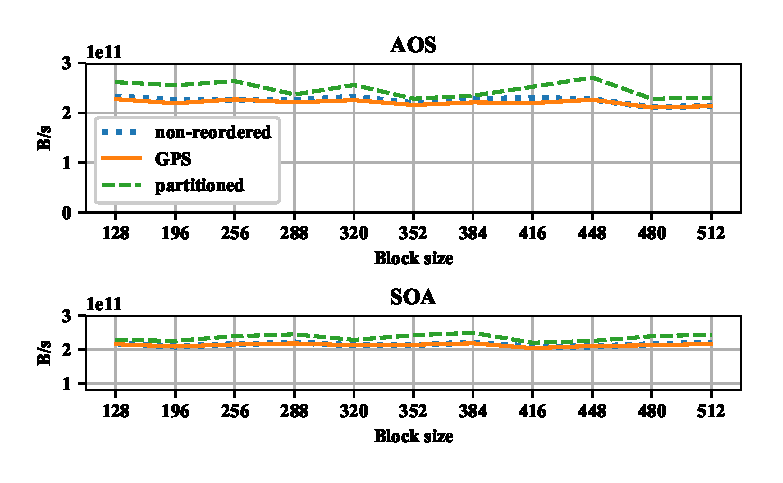
\includegraphics[width=9cm]{fig/airfoil_bw-vs-bs_hier_large.eps}
  \caption{\textbf{res\_calc} bandwidth on a dataset with $2880000$ cells with
  hierarchical colouring. Note that the y-axis doesn't start at the origin.}
  \label{fig:airfoil_bw-vs-bs_hier_large}
\end{figure}

\begin{figure}[Htbp]
  \centering
  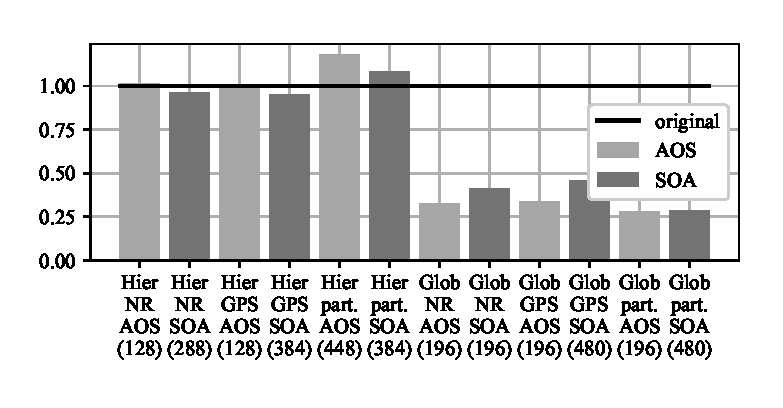
\includegraphics[width=9cm]{fig/airfoil_speedup_large.eps}
  \caption{\textbf{res\_calc} kernel speedup compared to the original code. Done
  on a dataset with $2800000$ cells. The block sizes are shown in parentheses,
  the reordering algorithms are: the original reordering (NR), GPS reordering
  and partitioning (part.)}
  \label{fig:airfoil_speedup_large}
\end{figure}

Although the number of block colours increased with reordering, it is only a
problem when the size of the dataset is so small that there are too few blocks for some colours to saturate the GPU.

When running on the newer Volta GPU architecture, the results look similar
(Figure \ref{fig:airfoil_bw-vs-bs_hier_large_volta}); the absolute value of the
bandwidths are (understandably) higher.

\begin{figure}[Htbp]
  \centering
  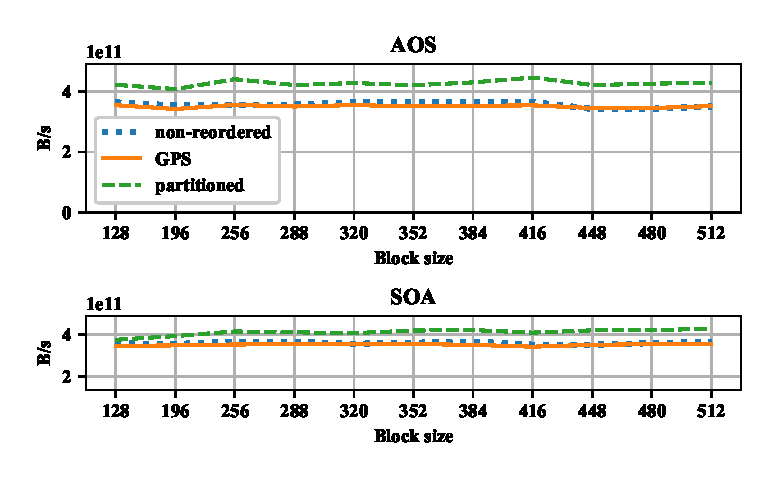
\includegraphics[width=9cm]{fig/airfoil_bw-vs-bs_hier_large_volta.eps}
  \caption{\textbf{res\_calc} bandwidth on a dataset with $2880000$ cells with
  hierarchical colouring, on Volta architecture. Note that the y-axis doesn't
  start at the origin.}
  \label{fig:airfoil_bw-vs-bs_hier_large_volta}
\end{figure}

On Volta, we achieved $1.28\times$ speedup in the kernel compared to the
original code with $446$ GB/s bandwidth ($60\%$ of the peak bandwidth). 
Since \textbf{res\_calc} takes around $54\%$ of the total run time in the
original code this speedup results in $1.14\times$ speedup on the
whole application.

\subsubsection{Analysis of Volna}

Measurements of the Volna application (\textbf{SpaceDiscretization} kernel)
with hierarchical colouring are shown in Figure \ref{fig:volna_bw-vs-bs_hier} and Table \ref{tab:volna_counters_hier}. The
reordering by partitioning again improves performance: it increases reuse from
$1.5$ to $2.8$ and decreases the number of global transactions by $18\%$ for
reads and $37\%$ for writes (Table \ref{tab:volna_counters_hier}). The larger
reduction in writes can be explained by the fact that the calculation does not
read the values of the indirect data from the previous iteration, only the
direct data.

Again, since the AoS version uses adjacent threads to load adjacent components
of data points, and also because one thread loads $4$ single precision values
into shared memory using the built-in vector type \lstinline!float4!, more data
can be transferred at the same time, thus there is a $2\%$ and $4\%$ reduction
in global memory transfers for reads and writes, respectively, leading to
increased performance ($292\,\text{GB/s}$ versus $268\,\text{GB/s}$).

Due to the low register counts ($28$--$32$) and the fact that volna uses float
(and int) datatypes compared to the doubles in Airfoil, the occupancy was quite
high (around $80\%$).  This explains the lack of dependence on the block size as
shown in the Figure \ref{fig:volna_bw-vs-bs_hier}.

Compared to Airfoil, the increase in the number of thread colours is less when
partitioning: from $3$ to $4$, hence, the synchronisation overhead is also less:
the percentage of stalls caused by synchronisation increases from $12\%$ to just
$15\%$. Of course, with high occupancy, the latency caused by synchronisation
can be better hidden by running warps from other blocks.

%shared memory usage:
% 7.7KB, 4.3 for metis

\begin{figure}[Htbp]
  \centering
  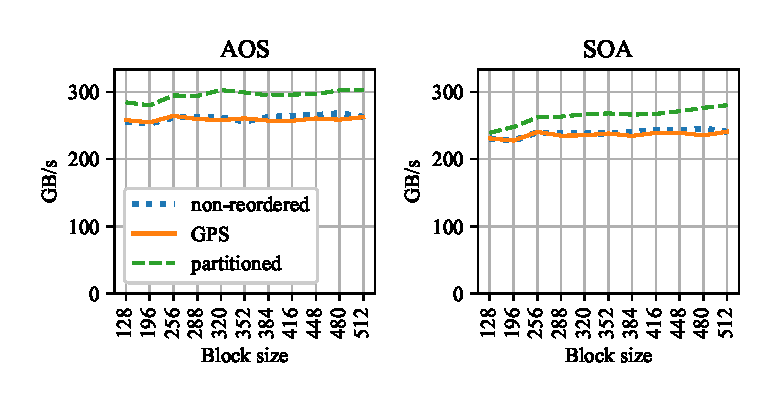
\includegraphics[width=9cm]{fig/volna_bw-vs-bs_hier.eps}
  \caption{\textbf{SpaceDiscretization} kernel bandwidth on a mesh with
  $3589735$ edges using hierarchical colouring. Note that the y-axis doesn't
  start at the origin.}
  \label{fig:volna_bw-vs-bs_hier}
\end{figure}

As can be seen from Figure \ref{fig:volna_speedup}, our implementation is $20\%$
faster than the original OP2 version. The $20\%$ performance gain in 
\textbf{SpaceDiscretization} results in $6\%$ increase regarding the whole 
application. The useful bandwidth also increased and reached $30\%$ of the peak 
stream bandwidth of the P100 GPU.

% volna counters {{{ %
% Block size: 448
% Hier:
%                                                      NR/AOS      NR/SOA     GPS/AOS     GPS/SOA   METIS/AOS   METIS/SOA
%                              Achieved Occupancy    0.819183    0.812192    0.815653    0.807516    0.796622    0.795811
%     Shared Memory Load Transactions Per Request    1.963101    1.963101    1.979188    1.979188    1.963848    1.963848
%    Shared Memory Store Transactions Per Request    1.961922    1.961922    1.978050    1.978050    1.973337    1.973337
%                   Device Memory Read Throughput  321.65GB/s  293.70GB/s  316.41GB/s  289.29GB/s  296.05GB/s  275.66GB/s
%                  Device Memory Write Throughput  86.010GB/s  80.508GB/s  85.125GB/s  80.088GB/s  60.913GB/s  59.338GB/s
%                        Shared Memory Efficiency      46.80%      46.80%      46.37%      46.37%      43.46%      43.46%
%                       Warp Execution Efficiency      98.21%      98.23%      98.19%      98.21%      96.98%      96.86%
%                            L2 Read Transactions     1843414     1858967     1536622     1551111      856125      871223
%                    L2 Read Transactions (total)     9217070     9294835     9219732     9306666     7705125     7841007
%                           L2 Write Transactions      495141      606426      413020      508079      150962      212536
%                   L2 Write Transactions (total)     2475705     3032130     2478120     3048474    13358658     1912814
%            Global Load Transactions Per Request    7.640348    7.339438    7.636162    7.336397    7.902319    7.678309
%           Global Store Transactions Per Request   16.172904    4.952004   16.187515    4.978461   15.811365    5.565519
%                 Device Memory Read Transactions     1822932     1833121     1519970     1529759      832512      846379
%         Device Memory Read Transactions (total)     9114660     9165605     9119820     9178554     7492608     7617411
%                Device Memory Write Transactions      487468      502498      408925      423507      171297      182190
%        Device Memory Write Transactions (total)     2437340     2512490     2453550     2541042     1541673     1639710
%                      Unified Cache Transactions     3654877     3744600     3045707     3120472     1881172     1917606
%              Unified Cache Transactions (total)    18274385    18274242    18274242    18722832    16930548    17258454
%           Issue Stall Reasons (Synchronization)      11.57%      11.72%      11.49%      11.60%      15.19%      14.60%
%              Issue Stall Reasons (Data Request)      50.79%      50.42%      50.14%      49.64%      45.80%      45.87%
%      Issue Stall Reasons (Execution Dependency)      16.93%      15.15%      17.00%      15.21%      16.41%      15.37%
%                                    Executed IPC    0.637022    0.630574    0.631593    0.625840    0.684925    0.661694
%                                      Issued IPC    0.638148    0.634302    0.633373    0.625643    0.686123    0.664217
%                                     Issue Slots     5963094     6515259     4972874     5433348     3101645     3319288
%                             Issue Slots (total)    29815470    32576295    29837244    32600088    27914805    29873592
%                          Issue Slot Utilization      27.35%      27.14%      27.15%      26.77%      29.39%      28.58%
%                         Multiprocessor Activity      95.44%      95.46%      93.98%      94.84%      92.02%      92.91%
%                 Eligible Warps Per Active Cycle    0.842456    0.842146    0.831790    0.828826    0.906572    0.878926
%                               Branch Efficiency      99.70%      99.70%      99.70%      99.70%     100.00%     100.00%
%        Warp Non-Predicated Execution Efficiency      94.27%      94.33%      94.25%      94.31%      92.74%      92.57%
%                    FLOP Efficiency(Peak Single)       1.64%       1.48%       1.60%       1.46%       1.68%       1.54%
%                    FLOP Efficiency(Peak Double)       0.00%       0.00%       0.00%       0.00%       0.00%       0.00%
%                   L2 Throughput (Texture Reads)  325.17GB/s  297.85GB/s  319.74GB/s  293.18GB/s  304.26GB/s  283.61GB/s
%                         Number of Block Colours           5           5           6           6           9           9
%                                    Reuse factor         1.5         1.5         1.5         1.5         2.8         2.8
%                       Average cache lines/block         300         307         300         308         165         184
%                        Number of Thread Colours           3           3           3           3           4           4
%                                       Bandwidth     265GB/s     241GB/s     260GB/s     238GB/s     292GB/s     268GB/s


% Glob:
%                                                   NR/AOS         NR/SOA     GPS/AOS     GPS/SOA   METIS/AOS   METIS/SOA
%                              Achieved Occupancy    0.766773    0.803794    0.769389    0.803205    0.766715    0.804845
%     Shared Memory Load Transactions Per Request    0.000000    0.000000    0.000000    0.000000    0.000000    0.000000
%    Shared Memory Store Transactions Per Request    0.000000    0.000000    0.000000    0.000000    0.000000    0.000000
%                   Device Memory Read Throughput  137.98GB/s  175.58GB/s  137.87GB/s  175.54GB/s  162.95GB/s  198.48GB/s
%                  Device Memory Write Throughput  66.312GB/s  92.108GB/s  66.360GB/s  92.292GB/s  76.224GB/s  100.73GB/s
%                        Shared Memory Efficiency       0.00%       0.00%       0.00%       0.00%       0.00%       0.00%
%                       Warp Execution Efficiency     100.00%     100.00%     100.00%     100.00%     100.00%     100.00%
%                            L2 Read Transactions     3874510     5586520     3886221     5599572     3230910     4083889
%                    L2 Read Transactions (total)    19372550    27932600    19431105    27997860    16154550    20419445
%                           L2 Write Transactions     5991159     4334428     6009907     4336008     5829332     3838742
%                   L2 Write Transactions (total)    29955795    21672140    30049535    21680040    29146660    19193710
%            Global Load Transactions Per Request   15.882479   13.241723   15.911647   13.244798   15.415391   12.327450
%           Global Store Transactions Per Request   31.580901   24.143615   31.673654   24.151083   30.845106   21.377642
%                 Device Memory Read Transactions     2790833     2409306     2793623     2410408     2653476     2414430
%         Device Memory Read Transactions (total)    13954165    12046530    13968115    12052040    13267380    12072150
%                Device Memory Write Transactions     1341294     1263924     1344665     1267340     1241239     1225405
%        Device Memory Write Transactions (total)     6706470     6319620     6723325     6336700     6206195     6127025
%                      Unified Cache Transactions     2871808     2961552     2871808     2961552     2871808     2961552
%              Unified Cache Transactions (total)    14359040    14807760    14359040    14807760    14359040    14807760
%           Issue Stall Reasons (Synchronization)       0.00%       0.00%       0.00%       0.00%       0.00%       0.00%
%              Issue Stall Reasons (Data Request)      13.80%      59.67%      13.83%      59.53%      14.96%      64.60%
%      Issue Stall Reasons (Execution Dependency)      21.13%      14.28%      21.12%      14.35%      20.87%      13.06%
%                                    Executed IPC    0.082505    0.144665    0.082124    0.144152    0.102872    0.162639
%                                      Issued IPC    0.082422    0.144362    0.082062    0.144732    0.103173    0.162981
%                                     Issue Slots     2585046     3194800     2585911     3194673     2585401     3194689
%                             Issue Slots (total)    12925230    15974000    12929555    15973365    12927005    15973445
%                          Issue Slot Utilization       3.27%       5.96%       3.25%       5.97%       4.09%       6.73%
%                         Multiprocessor Activity      97.28%      96.89%      97.23%      96.96%      96.20%      96.84%
%                 Eligible Warps Per Active Cycle    0.069532    0.130033    0.069495    0.130403    0.087902    0.150631
%                               Branch Efficiency     100.00%     100.00%     100.00%     100.00%     100.00%     100.00%
%        Warp Non-Predicated Execution Efficiency      97.92%      98.25%      97.92%      98.25%      97.92%      98.25%
%                    FLOP Efficiency(Peak Single)       0.39%       0.57%       0.39%       0.57%       0.48%       0.64%
%                    FLOP Efficiency(Peak Double)       0.00%       0.00%       0.00%       0.00%       0.00%       0.00%
%                   L2 Throughput (Texture Reads)  191.65GB/s  407.69GB/s  191.84GB/s  407.76GB/s  198.30GB/s  335.78GB/s
%                               Number of Colours           5           5           5           5           5           5
%                                       Bandwidth      82GB/s     116GB/s      82GB/s     116GB/s     102GB/s     128GB/s
% }}} volna counters %

%XXX: make this table look more like the airfoil one
\begin{table}[Htbp]
  \centering
  \resizebox{\columnwidth}{!}{
  \small
  % \begin{tabular}{|R{5.5cm}|cc|c|c|}
  \begin{tabular}{|r|cc|c|c||c|}
    \hline
      Reordering  & \multicolumn{2}{c|}{none} & \multicolumn{2}{c||}{partition} & original\\
      \hline
      Data layout &    AOS      &   SOA     &     AOS      &    SOA      &    SOA\\
      \hline
                               Bandwidth (GB/s) &   $ 133$ &   $ 120$ &   $ 146$ &   $ 134$ & $119$\\
                               Runtime (ms) & $0.87$ & $0.95$ & $0.77$ & $0.85$ & $0.93$\\
                             Achieved Occupancy &   $0.82$ &   $0.81$ &   $0.80$ &   $0.80$  &   $0.68$                                                    \\
        Global Memory Read Transactions &   $ 9114\text{k}$ &   $ 9166\text{k}$ &   $ 7493\text{k}$ &   $ 7617\text{k}$ &  $9504\text{k}$               \\
       Global Memory Write Transactions &   $ 2438\text{k}$ &   $ 2512\text{k}$ &   $ 1542\text{k}$ &   $ 1640\text{k}$ &   $ 2809\text{k}$           \\
                        Number of Block Colours &   $       5$ &   $       5$ &   $       9$ &   $       9$ &   $       6$                                   \\
                       Number of Thread Colours &   $       3$ &   $       3$ &   $       4$ &   $       4$ &   $       3$                                    \\
                                   Reuse factor &   $     1.5$ &   $     1.5$ &   $     2.8$ &   $     2.8$ &   $     1.48$                                    \\
          Issue Stall Reasons (Synchronization) &     $11\%$ &     $12\%$ &    $15\%$ &     $15\%$ &     $14\%$ \\
             Issue Stall Reasons (Data Request) &     $51\%$ &     $50\%$ &    $46\%$ &     $46\%$ &     $47\%$ \\
                      Average cache lines/block &   $     300$ &   $     307$ &   $     165$ &   $     184$ &   -                                \\
                      Warp Execution Efficiency &   $  98\%$ &   $  98\%$ &   $  97\%$ &   $  97\%$ &   $  65\%$                                            \\
      \hline
      Block size &  \multicolumn{4}{c||}{$307$} & $128$\\
    \hline
  \end{tabular}
  }
  \caption{Collected performance metrics of the hierarchical colouring
  implementation of the \textbf{SpaceDiscretization} kernel.}
  \label{tab:volna_counters_hier}
\end{table}


\begin{figure}[Htbp]
  \centering
  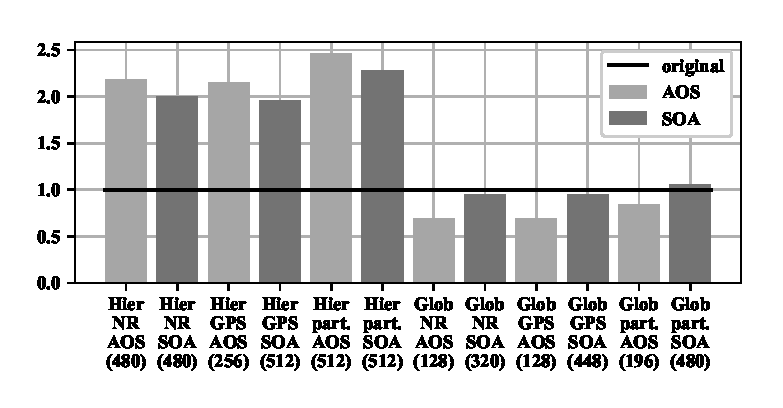
\includegraphics[width=9cm]{fig/volna_speedup.eps}
  \caption{\textbf{SpaceDiscretization} kernel speedup compared to the original
  code, done on a mesh with $3589735$ edges. The block sizes are shown in
  parentheses, the reordering algorithms are: the original reordering (NR), GPS
  reordering and partitioning (part.)}
  \label{fig:volna_speedup}
\end{figure}

On Volta, the performance of the kernel was $462$ GB/s ($62\%$ of the peak
bandwidth). Which means $1.18\times$ speedup on the kernel and $1.05\times$ 
speedup on the whole application compared to the original.



\subsubsection{Analysis of BookLeaf}

The measurements on the BookLeaf application (specifically the
\textbf{getacc\_scatter} kernel), as can be seen on Figures
\ref{fig:bookleaf_bw-vs-bs_hier} and \ref{fig:bookleaf_speedup}, also benefits
from the partitioning of the mesh.

The register count and occupancy are also similar to those with Airfoil ($64$
registers, achieving occupancy or around $40\%$), this leads to the variations
in performance along different block sizes.

With partitioning, the number of thread colours increased from $2$ to $5$, this
leads to the increased stalls from synchronisation: from $9\%$ to $20\%$, while
the reuse factor increases (from $2$ to $3.5$), which is comparable to that of
Airfoil, this explains the smaller increase in performance (only $9\%$, compared
to the $19\%$ increase in Airfoil).

The higher data reuse leads to $14\%$ and $41\%$ decrease of the number of
global transactions, for reads and writes, respectively. This large difference
between reads and writes is also because, like \textbf{SpaceDiscretization},
\textbf{getacc\_scatter} does not read values indirectly.

The best performance we achieved with \textbf{getacc\_scatter} results in  about
$2\%$ performance increase regarding the whole application. The useful bandwidth
also increased and reached $83\%$ of the peak stream bandwidth of the P100 GPU.

%shared mem: 17KB, with metis: 10.8


% bookleaf counters {{{ %
% Block size: 320
% Hier:                                                NR/AOS      NR/SOA     GPS/AOS     GPS/SOA   METIS/AOS   METIS/SOA
%                              Achieved Occupancy    0.430394    0.419929    0.430497    0.419961    0.434595    0.433032
%     Shared Memory Load Transactions Per Request    3.981157    3.289180    3.965366    3.279328    4.223552    3.869437
%    Shared Memory Store Transactions Per Request    3.317178    3.317178    3.313537    3.313537    3.884143    3.884143
%                   Device Memory Read Throughput  354.55GB/s  353.91GB/s  354.64GB/s  352.30GB/s  333.45GB/s  328.41GB/s
%                  Device Memory Write Throughput  104.92GB/s  105.59GB/s  104.86GB/s  105.02GB/s  67.486GB/s  69.298GB/s
%                        Shared Memory Efficiency      54.61%      60.09%      54.33%      59.75%      37.76%      39.35%
%                       Warp Execution Efficiency      99.50%      99.12%      99.38%      99.01%      95.70%      95.28%
%                            L2 Read Transactions     6811876     6855391     6809336     6852296     2636900     2676226
%                           L2 Write Transactions     2008024     2219229     2005901     2215992      509685      596673
%            Global Load Transactions Per Request    7.363423    7.884146    7.371714    7.880355    9.882201   10.026395
%           Global Store Transactions Per Request   15.672195    8.453975   15.672568    8.451264   15.785150    8.920493
%                 Device Memory Read Transactions     6792176     6810370     6789733     6807831     2588640     2616027
%                Device Memory Write Transactions     2010086     2031941     2007509     2029457      523903      552014
%                      Unified Cache Transactions     9270000     9153125     9267322     9150760     3651066     3644682
%           Issue Stall Reasons (Synchronization)       8.82%       9.02%       9.07%       9.45%      19.93%      20.05%
%              Issue Stall Reasons (Data Request)      74.74%      73.59%      74.26%      72.17%      58.52%      56.93%
%      Issue Stall Reasons (Execution Dependency)       6.73%       6.15%       6.76%       6.72%       8.03%       7.65%
%                                      Issued IPC    0.416526    0.360275    0.417040    0.395814    0.450024    0.424922
%                                     Issue Slots    14139389    13392697    14172617    13426925     6012129     5873760
%                          Issue Slot Utilization      18.71%      15.94%      18.72%      17.51%      20.02%      18.78%
%                 Eligible Warps Per Active Cycle    0.640313    0.549370    0.642497    0.608124    0.682836    0.655757
%                               Branch Efficiency      99.68%      99.66%      99.68%      99.66%      99.72%      99.68%
%        Warp Non-Predicated Execution Efficiency      96.92%      96.44%      96.81%      96.33%      93.02%      92.55%
%                    FLOP Efficiency(Peak Single)       0.00%       0.00%       0.00%       0.00%       0.00%       0.00%
%                    FLOP Efficiency(Peak Double)       1.63%       1.47%       1.62%       1.61%       1.63%       1.56%
%                   L2 Throughput (Texture Reads)  355.56GB/s  356.23GB/s  355.65GB/s  354.56GB/s  339.58GB/s  335.89GB/s
%                                    Executed IPC    0.416240    0.359758    0.416665    0.395579    0.452258    0.424822
%                         Multiprocessor Activity      98.40%      98.68%      98.39%      98.64%      95.56%      95.75%
%                         Number of Block Colours           4           4           4           4           9           9
%                                    Reuse Factor           2           2           2           2         3.5         3.5
%                       Average Cache Lines/Block         643         648         642         648         367         390
%                        Number of Thread Colours           2           2         2.1         2.1           5           5
%                                       Bandwidth     377GB/s     375GB/s     377GB/s     374GB/s     412GB/s     401GB/s
% }}} bookleaf counters %

\begin{figure}[Htbp]
  \centering
  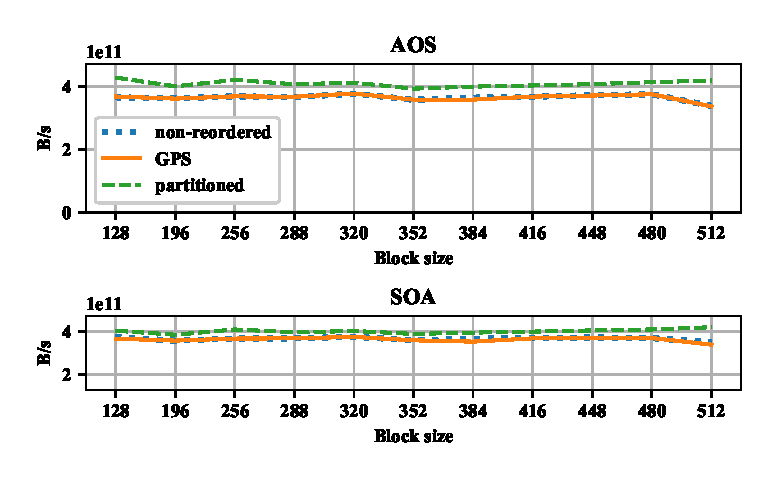
\includegraphics[width=9cm]{fig/bookleaf_bw-vs-bs_hier.eps}
  \caption{\textbf{getacc\_scatter} kernel bandwidth on a mesh with $4000000$
  edges using hierarchical colouring. Note that the y-axis doesn't start at the
  origin.}
  \label{fig:bookleaf_bw-vs-bs_hier}
\end{figure}

\begin{figure}[Htbp]
  \centering
  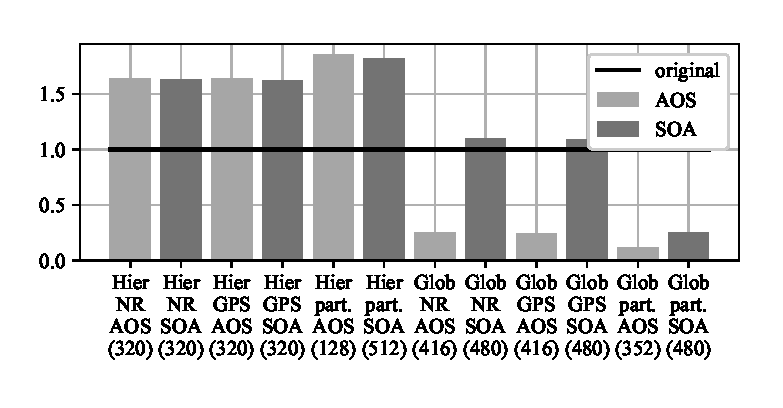
\includegraphics[width=9cm]{fig/bookleaf_speedup.eps}
  \caption{\textbf{getacc\_scatter} kernel speedup compared to the original
  code, done on a mesh with $4000000$ edges. The block sizes are shown in
  parentheses, the reordering algorithms are: the original reordering (NR), GPS
  reordering and partitioning (part.)}
  \label{fig:bookleaf_speedup}
\end{figure}

On Volta, the performance of the kernel was $631$ GB/s ($85\%$ of the peak
bandwidth which results in $1.03\times$ speedup on the whole application compared
to the original.


\subsubsection{Analysis of LULESH}\label{sec:analysis-of-lulesh}


The \textbf{IntegrateStressForElems} kernel uses a mapping with 8 neighbours
(compared to the 2--4 as in the case of the previous ones) for the brick
elements. Due to this, the number of colours is quite high: $8$, $16$ and $24$
in the global coloring versions (for the different reorderings), and $4$, $50$
and $15$ in the hierarchical colouring versions. The number of thread colours
was also quite high: $4$ in the non-reordered ($4.5$ in the GPS) and $11.6$ in
the partitioned version: this is a much higher increase compared to the previous
applications (Table \ref{tab:lulesh_counters_hier}). At the same time of course,
data reuse is higher compared to 2D applications - between $2.6$ and $4.8$.

The other aspect in which LULESH is different is that it uses a high amount of
registers ($96$), significantly decreases occupancy: with block size 320, the
AoS version achieved $15\%$ and the SoA version achieved around $30\%$.

Because of these two reasons, the synchronisation overhead ($39\%$ stalls were
from synchronisation on the partitioned mesh) couldn't be hidden: there were no
warps from other blocks to be scheduled in place of the stalled ones because
there was only one block running on each multiprocessor. The difference in
achieved occupancy also means that the SoA version with two blocks per
multiprocessor performs better.

\begin{figure}[Htbp]
  \centering
  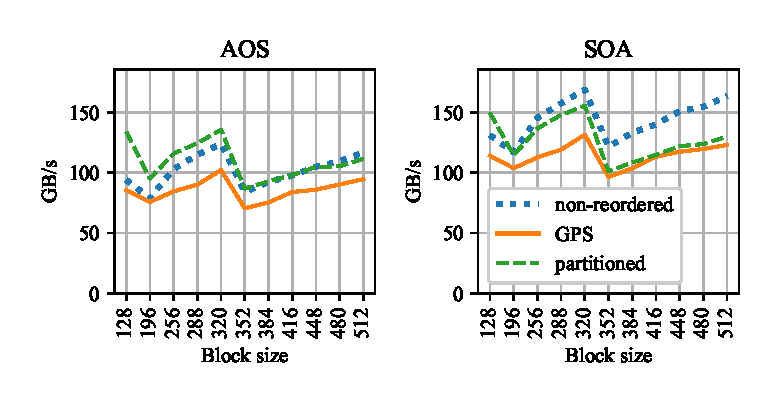
\includegraphics[width=9cm]{fig/lulesh_bw-vs-bs_hier.eps}
  \caption{\textbf{IntegrateStressForElems} kernel bandwidth on a mesh with
  $4913000$ cells using hierarchical colouring. Note that the y-axis doesn't
  start at the origin.}
  \label{fig:lulesh_bw-vs-bs_hier}
\end{figure}

Nevertheless, as shown on Figure \ref{fig:lulesh_speedup}, our hierarchical
colouring algorithm performs significantly better than the original, two-step
implementation, and also uses much less memory. Although the original needs less
synchronisation, the resulting warp divergence also cannot be hidden if the
occupancy is this low.

In the original version $37\%$ of the total time is spent in
\textbf{IntagrateStressForElems}, therefore the achieved $1.75\times$ speedup on
the kernel causes about $1.28\times$ speedup on the whole application. The
useful bandwidth in case of the best version of \textbf{IntegrateStressForElems}
reached $20\%$ of the peak stream bandwidth of the P100 GPU.

% lulesh counters {{{ %
% Block size: 320
% Hier:
%                                                      NR/AOS      NR/SOA     GPS/AOS     GPS/SOA   METIS/AOS   METIS/SOA
%                              Achieved Occupancy    0.153342    0.293920    0.153550    0.284203    0.153820    0.299256
%     Shared Memory Load Transactions Per Request    3.813638    3.526038    4.002716    3.631602    4.479968    4.322711
%    Shared Memory Store Transactions Per Request    3.316784    2.944442    3.508397    3.034623    3.742974    3.536361
%                   Device Memory Read Throughput  117.78GB/s  276.24GB/s  100.31GB/s  214.79GB/s  74.064GB/s  155.87GB/s
%                  Device Memory Write Throughput  44.459GB/s  99.108GB/s  38.989GB/s  79.804GB/s  26.038GB/s  54.191GB/s
%                        Shared Memory Efficiency      48.54%      53.36%      45.44%      50.98%      30.47%      31.81%
%                       Warp Execution Efficiency      97.64%      96.94%      97.39%      96.41%      91.39%      89.82%
%                            L2 Read Transactions     8927298     8925744      733415      739319     1621952     1715366
%                    L2 Read Transactions (total)    35709192    35702976    36670750    36965950    24329280    25730490
%                           L2 Write Transactions     3429290     3433123      281319      288606      574252      631224
%                   L2 Write Transactions (total)    13717160    13732492    14065950    14430300     8613780     9468360
%            Global Load Transactions Per Request    8.461524    9.445318    8.365310    9.635046    8.782532    9.537800
%           Global Store Transactions Per Request    8.659927    8.668800    8.650857    8.798241    9.222445   10.001870
%                 Device Memory Read Transactions     8393075     8851961      690624      727464     1525893     1668476
%         Device Memory Read Transactions (total)    33572300    35407844    34531200    36373200    22888395    25027140
%                Device Memory Write Transactions     3168271     3175906      268437      270294      536445      580062
%        Device Memory Write Transactions (total)    12673084    12703624    13421850    13514700     8046675     8700930
%                      Unified Cache Transactions    12854357    11281423     1048169      918060     2389410     2202778
%              Unified Cache Transactions (total)    51417428    45125692    52408450    45903000    35841150    33041670
%           Issue Stall Reasons (Synchronization)      13.27%      19.06%      14.11%      17.78%      39.46%      41.75%
%              Issue Stall Reasons (Data Request)      63.80%      56.40%      61.52%      55.14%      34.65%      30.51%
%      Issue Stall Reasons (Execution Dependency)      12.35%      10.16%      12.52%      10.18%      14.20%      12.85%
%                                    Executed IPC    0.316365    0.514800    0.319681    0.472282    0.295742    0.488715
%                                      Issued IPC    0.316544    0.513558    0.320049    0.473822    0.295894    0.490463
%                                     Issue Slots    46704488    32475988     3815312     2649675    11050475     9059009
%                             Issue Slots (total)   186817952   129903952   190765600   132483750   165757125   135885135
%                          Issue Slot Utilization      15.03%      23.13%      15.19%      21.32%      13.79%      22.20%
%                         Multiprocessor Activity      98.82%      98.50%      89.85%      90.13%      96.44%      94.58%
%                 Eligible Warps Per Active Cycle    0.587770    1.128024    0.588915    1.037127    0.550260    1.021502
%                               Branch Efficiency      99.36%      99.12%      99.42%      99.21%      99.41%      99.32%
%        Warp Non-Predicated Execution Efficiency      96.62%      95.45%      96.40%      94.95%      90.27%      88.38%
%                    FLOP Efficiency(Peak Single)       0.00%       0.00%       0.00%       0.00%       0.00%       0.00%
%                    FLOP Efficiency(Peak Double)       5.16%      11.43%       4.65%       9.42%       5.16%       9.91%
%                   L2 Throughput (Texture Reads)  125.25GB/s  278.49GB/s  106.33GB/s  217.85GB/s  78.652GB/s  160.10GB/s
%                         Number of Block Colours           4           4          50          50          15          15
%                                    Reuse Factor         2.6         2.6         2.5         2.5         4.8         4.8
%                       Average Cache Lines/Block         744         747         770         781         427         474
%                        Number of Thread Colours           4           4         4.5         4.5        11.6        11.6
%                                       Bandwidth     124GB/s     168GB/s     102GB/s      94GB/s     129GB/s     147GB/s
% }}} lulesh counters %

\begin{figure}[Htbp]
  \centering
  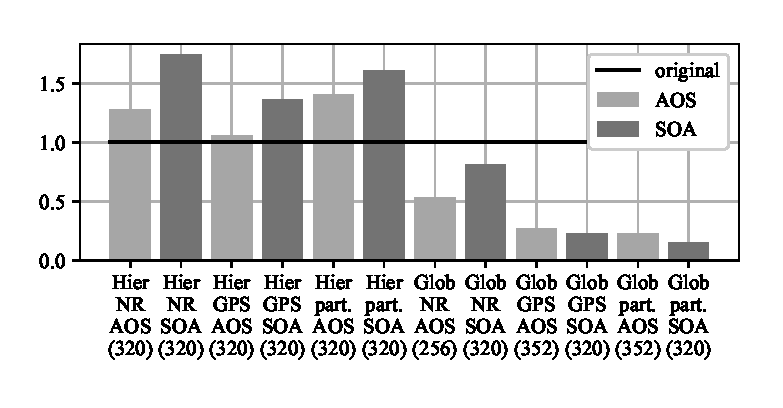
\includegraphics[width=9cm]{fig/lulesh_speedup.eps}
  \caption{\textbf{IntegrateStressForElems} kernel speedup compared to the
  original (gathering) code, done on a mesh with $4913000$ cells. The block
  sizes are shown in parentheses, the reordering algorithms are: the original
  reordering (NR), GPS reordering and partitioning (part.)}
  \label{fig:lulesh_speedup}
\end{figure}

\begin{table}[Htbp]
  \centering
  \resizebox{\columnwidth}{!}{
  % \begin{tabular}{|R{2.5cm}|cc|c|c|}
    \small
  \begin{tabular}{|r|cc|c|c||c|}
    \hline
      Reordering  & \multicolumn{2}{c|}{none} & \multicolumn{2}{c||}{partition} & original\\
      \hline
      Data layout &    AOS      &   SOA     &     AOS      &    SOA & SOA\\
      \hline
                               Bandwidth (GB/s) &   $ 124$ &   $ 168$ &   $ 129$ &   $ 147$ & $97$\\
                               Runtime (ms)     &   $5.45$ & $4.00$ & $4.98$ & $4.34$ & $6.98$ \\
                             Achieved Occupancy &   $0.15$ &   $0.29$ &   $0.15$ &   $0.30$ & $0.24$\\
        Global Memory Read Transactions (total) &   \num{33572}k & \num{35408}k &   \num{22888}k &   \num{25027}k  & \num{16072}k\\
       Global Memory Write Transactions (total) &   \num{12673}k & \num{12704}k &   \num{ 8047}k &   \num{ 8701}k  & \num{32689}k\\
                        Number of Block Colours &   $       4$ &   $       4$ & $      15$ &   $      15$ & - \\
                       Number of Thread Colours &   $       4$ &   $       4$ & $    11.6$ &   $    11.6$  & -\\
                                   Reuse Factor &   $     2.6$ &   $     2.6$ & $     4.8$ &   $     4.8$ & -\\
          Issue Stall Reasons (Synchronization) &   $  13\%$ &   $  19\%$ &   $ 39\%$ &   $  42\%$  & $0\%$\\
             Issue Stall Reasons (Data Request) &   $  64\%$ &   $  56\%$ &   $ 35\%$ &   $  31\%$  & $26\%$\\
                      Average Cache Lines/Block &   $     744$ &   $     747$ & $     427$ &   $     474$  & -\\
                      Warp Execution Efficiency &   $  98\%$ &   $  97\%$ &   $ 91\%$ &   $  90\%$ & $100\%$\\
      \hline
      Block size & \multicolumn{4}{c||}{$320$} & $64$\\

    \hline
  \end{tabular}
  }
  \caption{Collected performance metrics of the hierarchical colouring
    implementation of the \textbf{IntegrateStressForElems} kernel. The last
    column is the measured performance of the original code.}
  \label{tab:lulesh_counters_hier}
\end{table}

% TODO reformulate this paragraph
On Volta, we achieved $1.84\times$ speedup in the kernel compared to the
original code with $273$ GB/s bandwidth ($37\%$ of the peak bandwidth). In the
original version $35\%$ of the total time is spent in
\textbf{IntegrateStressForElems}, therefore the achieved kernel speedup causes
about $1.29\times$ speedup on the whole application.

\subsubsection{Analysis of miniAero}

The \textbf{compute\_face\_flux} kernel is the most computationally intensive
among the ones we tested: it uses $165$ registers in hierarchical  colouring
($166$ in SoA layout). Also, it achieves (with block size $384$ and reordered by
GPS) $15\%$ of peak double precision efficiency, compared to the $6$--$7\%$ in
Airfoil (Table \ref{tab:mini_aero_counters_hier}). It also uses $8$ square root
operations and several divides that can't efficiently fill the pipelines at such
low occupancy.

The amount of data indirectly accessed by the kernel is also large: each thread
accesses $2$ data points indirectly, each holding $32$ double precision values.
If all of that is loaded into shared memory, the size of it exceeds the hardware
limits with block sizes larger than $288$; it didn't run with the original mesh
numbering with any block size, and only with smaller block sizes on the reordered meshes (Figure \ref{fig:mini_aero_bw_crash}). The other measurements were carried out
by only loading the incremented data into shared memory.

\begin{figure}[Htbp]
  \centering
  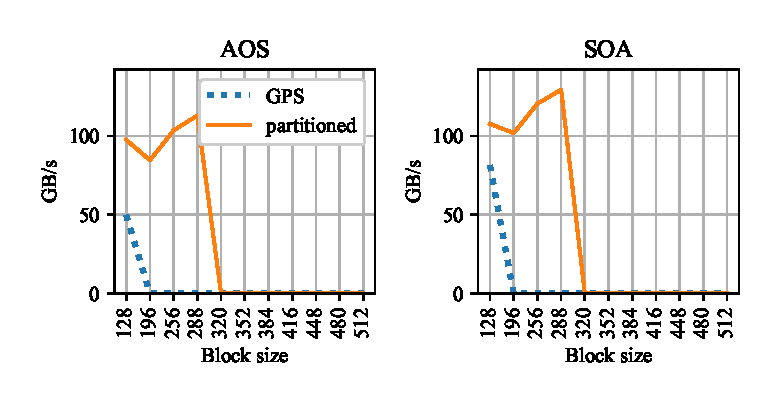
\includegraphics[width=9cm]{fig/mini_aero_bw_crash.eps}
  \caption{The \textbf{compute\_face\_flux} kernel bandwidth on a mesh with
  $6242304$ faces. The kernel didn't run in the cases where the data reuse was
  not high enough because the large amount of shared memory needed; these are
  shown here with $0$ bandwidth.}
  \label{fig:mini_aero_bw_crash}
\end{figure}

The mesh also has a complex structure ($18$ and $15$ block colours for GPS
reordered and partitioned versions, respectively) and the original ordering was
far from optimal: we couldn't run the non-reordered version, because the number
of block colours exceeded the implementation limit of the library, which is
$256$.

As with LULESH, only one block was running at a time on each multiprocessor.
Although the synchronisation overhead was lower ($3$ and $6$ thread
colours in the GPS reordered and partitioned versions, respectively), the costly
operations prevented high performance gains in the case of the partitioned
version (Figure \ref{fig:mini_aero_bw_small-cache}).

\begin{figure}[Htbp]
  \centering
  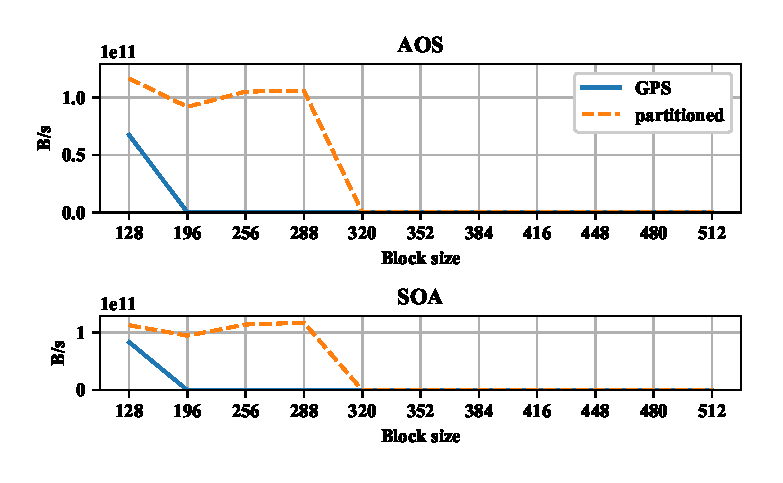
\includegraphics[width=9cm]{fig/mini_aero_bw_small-cache.eps}
  \caption{The \textbf{compute\_face\_flux} kernel bandwidth on a mesh with
  $6242304$ faces. The shared memory was only used to cache the increments,
  reducing the need for large shared memory size. The kernel didn't fit into the
  shared memory with block size larger than $384$ or if not reordered because
  the large amount of shared memory needed; these are shown here with $0$
  bandwidth.}
  \label{fig:mini_aero_bw_small-cache}
\end{figure}

The original Kokkos implementation either used atomic adds or the two-step
gathering approach depending on compilation parameters. Our implementation
outperformed both (Figure \ref{fig:mini_aero_speedup_small-cache}), for the same
reason as in case of LULESH.

In the original version $22\%$ of the total time is spent in
\textbf{compute\_face\_flux}, therefore the achieved $1.22\times$ kernel speedup
causes about $1.04\times$ speedup on the whole application. The useful bandwidth
in case of the best version of \textbf{compute\_face\_flux} ($117$ GB/s) reached
$24\%$ of the peak stream bandwidth of the P100 GPU.

% mini_aero counters {{{ %
% Block size: 128
% Hier:                                            GPS/AOS        GPS/SOA   METIS/AOS   METIS/SOA
%                              Achieved Occupancy    0.061617    0.060943    0.121864    0.121086
%     Shared Memory Load Transactions Per Request    3.089353    2.930011    4.559967    4.435671
%    Shared Memory Store Transactions Per Request    4.597106    2.132409    4.931486    2.612757
%                   Device Memory Read Throughput  84.899GB/s  154.47GB/s  113.68GB/s  185.10GB/s
%                  Device Memory Write Throughput  10.564GB/s  19.753GB/s  14.249GB/s  21.629GB/s
%                        Shared Memory Efficiency      49.82%      66.99%      33.81%      40.56%
%                       Warp Execution Efficiency      91.41%      84.43%      88.06%      85.42%
%                            L2 Read Transactions     3746994     4192153     3322917     4813039
%                    L2 Read Transactions (total)    74939880    83843060    56489589    81821663
%                           L2 Write Transactions      450646      544462      374918      576190
%                   L2 Write Transactions (total)     9012920    10889240     6373606     9795230
%            Global Load Transactions Per Request    8.363060    9.608935    9.101123   11.272758
%           Global Store Transactions Per Request    8.928965    8.552480   10.217068   13.250228
%                 Device Memory Read Transactions     3678059     4101386     3141355     4534744
%         Device Memory Read Transactions (total)    73561180    82027720    53403035    77090648
%                Device Memory Write Transactions      457662      524480      393745      529889
%        Device Memory Write Transactions (total)     9153240    10489600     6693665     9008113
%                      Unified Cache Transactions     5026525     4529910     4429316     4059892
%              Unified Cache Transactions (total)   100530500    90598200    75298372    69018164
%           Issue Stall Reasons (Synchronization)       4.33%       8.66%      15.13%      20.92%
%              Issue Stall Reasons (Data Request)      60.60%      35.22%      47.30%      34.50%
%      Issue Stall Reasons (Execution Dependency)      23.06%      32.73%      22.71%      23.30%
%                                    Executed IPC    0.252724    0.375217    0.472362    0.496491
%                                      Issued IPC    0.253601    0.375074    0.472305    0.496602
%                                     Issue Slots    22380958    19376361    23994392    21907800
%                             Issue Slots (total)   447619160   387527220   407904664   372432600
%                          Issue Slot Utilization      11.90%      16.92%      21.96%      22.51%                                                 
%                         Multiprocessor Activity      98.16%      97.83%      98.53%      98.68% 
%                 Eligible Warps Per Active Cycle    0.265263    0.383198    0.534554    0.552878
%                               Branch Efficiency      99.45%      99.42%      99.42%      99.31%
%        Warp Non-Predicated Execution Efficiency      90.54%      83.43%      87.06%      84.18%
%                    FLOP Efficiency(Peak Double)       4.95%       8.38%       9.77%      11.50%
%                   L2 Throughput (Texture Reads)  86.394GB/s  157.71GB/s  120.09GB/s  196.28GB/s
%                         Number of Block Colours         20          20          17          17
%                                    Reuse Factor       1.98        1.98        3.26        3.26
%                       Average Cache Lines/Block        169         189         116         179
%                        Number of Thread Colours          3           3           6           6
%                                       Bandwidth
% }}} mini_aero counters %

\begin{figure}[Htbp]
  \centering
  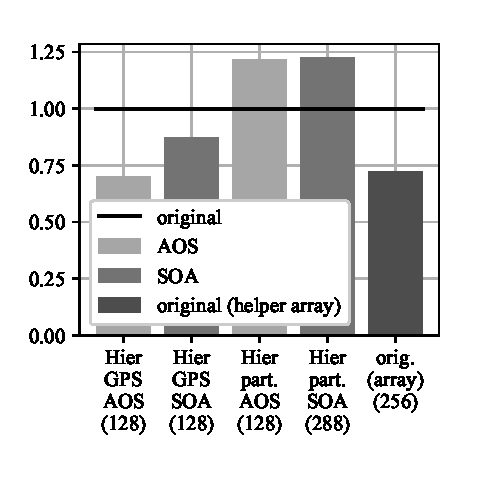
\includegraphics{fig/mini_aero_speedup_nocache.eps}
  \caption{The \textbf{compute\_face\_flux} kernel speedup compared to the
  original code that was using atomic adds, on a mesh with
  $6242304$ faces. The shared memory was only used to cache the increments,
  reducing the need for large shared memory size. The last bar shows the
  relative performance of the original code with the helper array approach.}
  \label{fig:mini_aero_speedup_small-cache}
\end{figure}

\begin{table}[Htbp]
  \centering
  \resizebox{\columnwidth}{!}{
    \small
  % \begin{tabular}{|R{2.5cm}|cc|c|c|}
  \begin{tabular}{|r|cc|c|c||c|}
    \hline
      Reordering  & \multicolumn{2}{c|}{GPS} & \multicolumn{2}{c||}{partition} & original\\
      \hline
      Data layout &    AOS      &   SOA     &     AOS      &    SOA & SOA\\
      \hline
                               Bandwidth (GB/s)&    $  67$ &   $ 84$ &   $ 117$ &   $ 113$ & $96$\\
                               Runtime (ms)    &    $19.09$ & $15.38$ & $11.04$
                               & $11.38$ & $13.39$\\
                             Achieved Occupancy&    $0.06$ & $0.06$ & $0.12$ & $0.12$  & $0.23$\\
                Global Memory Read Transactions&    $73561\text{k}$ & $82028\text{k}$ & $53403\text{k}$ & $77091\text{k}$  & $87368\text{k}$\\
               Global Memory Write Transactions&    $9153\text{k}$ & $10390\text{k}$ & $6694\text{k}$ & $9008\text{k}$ & $5934\text{k}$ \\
                        Number of Block Colours&    $      18$ &   $      18$ & $      15$ &   $      15$  & -\\
                       Number of Thread Colours&    $       3$ &   $       3$ & $       6$ &   $       6$  & -\\
                                   Reuse Factor&    $     2.2$ &   $     2.2$ & $     3.9$ &   $     3.9$  & -\\
          Issue Stall Reasons (Synchronization)&    $4\%$ & $9\%$ & $15\%$ & $21\%$    & $0\%$ \\
             Issue Stall Reasons (Data Request)&    $61\%$ & $35\%$ & $47\%$ & $35\%$  & $49\%$\\
     Issue Stall Reasons (Execution Dependency)&    $23\%$ & $33\%$ & $23\%$ & $23\%$  & $13\%$\\
                      Average Cache Lines/Block&    $     452$ &   $     471$ & $     269$ &   $     344$  & -\\
                      Warp Execution Efficiency&    $91\%$ & $84\%$ & $88\%$ & $85\%$  & $91\%$\\
                   FLOP Efficiency(Peak Double)&    $5\%$ & $8\%$ & $10\%$ & $12\%$  & $8\%$\\
      \hline
      Block size & \multicolumn{4}{c||}{128} & 256\\
    \hline
  \end{tabular}
  }
  \caption{Collected performance metrics of the hierarchical colouring
    implementation of the \textbf{compute\_face\_flux} kernel. The last column
    is the measured performance of the original code.}
  \label{tab:mini_aero_counters_hier}
\end{table}

% TODO reformulate this paragraph
On Volta, we achieved $1.87\times$ speedup in the kernel compared to the
original code with $263$ GB/s bandwidth ($35\%$ of the peak bandwidth). In the
original version $27\%$ of the total time is spent in
\textbf{compute\_face\_flux}, therefore the kernel speedup causes about
$1.24\times$ speedup on the whole application.


\subsubsection{Analysis of structured meshes}

As mentioned in Sections \ref{sec:mini-aero-summary} and
\ref{sec:lulesh-summary}, the meshes of miniAero and LULESH are actually structured meshes, generated by the
code itself. This lets us to use the structured nature of the mesh to create partitions with netter shapes than what METIS produces. This in turn allows us to understand the trade-off between
high data reuse and few thread colours used more by creating 1D, 2D and 3D
partitions (these will have an increasing amount of reuse and number of colours).

While both kernels operate on 3D Cartesian (hex8) meshes, the
\textbf{IntegrateStressForElems} kernel in LULESH uses a mapping from cells to their
connected vertices, and the \textbf{compute\_face\_flux} kernel in miniAero maps from
(internal) faces to cells. We then created a number of different partition shapes - 1D lines, 2D rectangles and 3D bricks.

%In the former case, the blocks are created from the
%cells as rectangles.
% In the second case, the creation starts the same way, but at the last axis (the
% contiguous axis) three faces corresponding to one cell are added to the block at
% the same time. This way the blocks cover the whole mesh similarly to the
% previous case. This also means that when the block is long along the third axis,
% the reuse will be higher than it would be with the other two axes. Because of
% this, in our measurements, we ordered the dimensions of the blocks so that they
% are longest along this axis.

Figures \ref{fig:lulesh_block} and \ref{fig:mini_aero_block} show the
bandwidths, reuse factors and the number of thread colours across different
block-shapes, along with the result of partitioning the same mesh using METIS.
The size of the blocks is $128$. These measurements were run on meshes with
shape specifically tailored so that the handcrafted blocks can cover them
without any gaps.

In \textbf{IntegrateStressForElems}, the bandwidth of the original ordering achieved  $134\,\text{GB/s}$ - it uses a row major order, similar to ours
when we use a block shape that is $128$ cells long and only $1$ cell thin in the
other dimensions. The partitioned mesh (detailed
in Section \ref{sec:analysis-of-lulesh}) achieved $132\,\text{GB/s}$, and we achieved $167\,\text{GB/s}$
bandwidth using our handcrafted blocks, for the same block size ($128$). Note
that using regular shapes is better for the thread colouring algorithm too: with
METIS partitioning, the number of colours needed is higher than in the other
cases.

For \textbf{compute\_face\_flux}, we achieved $167\,\text{GB/s}$ bandwidth,
compared to $101\,\text{GB/s}$ achieved with METIS partitioning.

Of course, using these handcrafted blocks can only be done on meshes that are actually structured, therefore this is not representative of realistic cases. However, these results illustrate clearly that when
the number of thread colours are the same, increased reuse leads to better
performance. Also, there is an optimal number of thread colours for each
application, and performance will suffer above that. The challenge lies in
finding a partitioning algorithm that can either find the middle ground, or can
be tuned along the amount of reuse it aims to achieve. Such partitioning algorithms are not currently available, but we demonstrate a clear need for them.

\begin{figure}[Htbp]
  \centering
  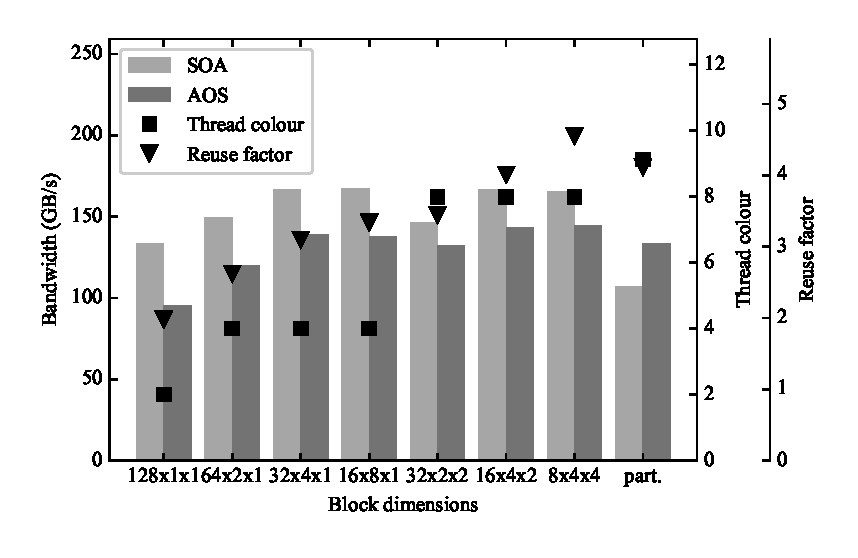
\includegraphics[width=12cm]{fig/lulesh_block.eps}
  \caption{\textbf{IntegrateStressForElems} kernel with explicitly controlled
  partitioning. For comparison, the last column shows the result on the same
  mesh, partitioned by METIS.}
  \label{fig:lulesh_block}
\end{figure}

\begin{figure}[Htbp]
  \centering
  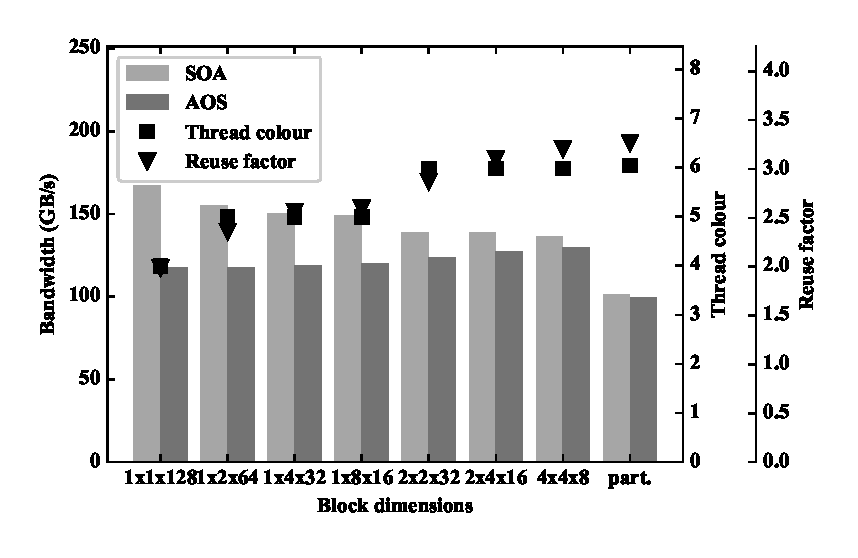
\includegraphics[width=12cm]{fig/mini_aero_block.eps}
  \caption{\textbf{compute\_face\_flux} kernel with explicitly controlled
  partitioning. For comparison, the last column shows the result on the same
  mesh, partitioned by METIS.}
  \label{fig:mini_aero_block}
\end{figure}

% vim:set et sw=2 ts=2 tw=80 fdm=marker:


\section{Conclusion}\label{conclusion}

We investigated the methods of accelerating parallel scientific computations on
unstructured meshes. We specifically looked at improving the performance of
memory-bound implementations executing on GPUs.

We designed a reordering algorithm which uses k-way recursive partitioning to
improve data reuse and with it, performance of unstructured mesh applications
accelerated on GPU platforms.

We implemented a library that can automatically (without major modifications
from the part of the user) parallelise serial user code, avoiding data races
using global and hierarchical colouring. It uses optimisations specifically
targeting GPUs, such as caching in shared memory, reordering by colours to
reduce warp divergence and using vector types to more efficiently utilise
available global memory bandwidth.

Using this library, we analysed the performance of our algorithms on a number of
representative unstructured mesh applications varying a number of parameters,
such as the different thread block sizes and data layouts (Array of Structs
versus Struct of Arrays).

When comparing the performance of global and hierarchical colouring (shared
memory caching) approach, the shared memory approach consistently performed
better, since it could exploit the temporal locality in indirectly accessed data
by avoiding data races in shared memory with synchronisation within thread
blocks rather than different kernel launches.

We also analysed the performance of reordering based on GPS renumbering and
partitioning. The former improves global colouring with increasing spatial
reuse, while the latter can significantly improve the shared memory approach by
increasing data reuse within thread blocks, which results in smaller shared
memory and fewer global memory transactions.

We have shown that there is a trade-off between high data reuse and large
numbers of thread colours in hierarchical colouring that is especially
pronounced when the achieved occupancy is low: the more thread colours a block
has, the more synchronisations it will need, the latency of which can be hard to
hide when there are few eligible warps.

Using our methods, we were able to achieve performance gains of $10\%$
(Airfoil), $140\%$ (Volna), $75\%$ (Bookleaf), $75\%$ (Lulesh) and $25\%$
(miniAero) over the original implementations. These results significantly
advance the state of the art, demonstrating that the algorithmic patterns used
in most current implementations (particularly in case of US DoE codes
represented by LULESH and MiniAero) could be significantly improved upon by the
adoption of two-level colouring schemes and partitioning for increased data
reuse.

When carrying out this work, it had become clear that partitioning algorithms in
traditional libraries such as Metis and Scotch weren't particularly well suited
for producing such small partition sizes. As potential future work, we wish to
explore algorithms that are better optimised for this purpose. The performance
of these partitioning algorithms was also low - parallelising this could be
another interesting challenge. Finally, we are planning to integrate these
algorithms into the OP2 library, so they can be automatically deployed on
applications that already use the OP2 library, such as Airfoil, BookLeaf, Volna
or Rolls-Royce Hydra.

% vim:set et sw=2 ts=2 tw=80:
